\section{Space efficient recursive partitioning}
\label{sec:algexpdec}

\noindent
The main goal of this section is to show Theorems~\ref{th:main} and~\ref{th:mainpoly}, restated here for convenience.

\mainbld*
\mainbldpoly*
\noindent
The only difference between the algorithms of Theorem~\ref{th:main} and~\ref{th:mainpoly} lies in the balanced sparse cut subroutine that they employ. Therefore, we present and analyse them in a unified manner by deferring the choice of the balanced sparse cut algorithm to later. Using the results from \cref{sec:spars} and \cref{sec:balsparse} (i.e. \cref{lem:distrcutstreamadd} and \cref{lem:reduction} respectively), we prove the following.


\begin{restatable}[Unified algorithm]{lemma}{unified}
	\label{lem:tech}
	Let $G=(V,E)$ be a graph given in a dynamic stream, let $b \in (0,1)$ be a parameter such that $b \le {1}/{\log n}$. Let $\bsc$ be an $(\alpha,\lambda)$-BSCA where \smash{$\alpha \le \frac{1}{b\log n}$} and \smash{$\lambda= O(1)$}. Also let $k$ be an integer such that \smash{$ k \ge {\log {(n^5 \alpha )} }/{ \log  {(b^{-1/2}}/{\lambda})} $}, and $k \le \log n$. Then there is an algorithm that maintains a linear sketch of $G$ in $\otil( n/b^3) \cdot \alpha^{O(k)}$ space. For all $\epsilon \in [n^{-2},b\log n]$, the algorithm decodes the sketch using $\bsc$ to compute, with high probability, a $(b,\epsilon,\phi,\gamma)$-BLD of $G$ for
	\begin{equation*}
		\phi = \Omega\left(\frac{\epsilon}{\alpha \log n}\right) \quad \text{ and } \quad \gamma = O(\alpha^{k+1}) \, .
	\end{equation*}
	Moreover, the decoding runs in $\otil( n/b^3) \cdot \alpha^{O(k)}+S(n,\otil( n/b^2) \cdot \alpha^{O(k)})$ space and  {$T(n,\otil( n/b^2) \cdot \alpha^{O(k)}) \cdot \poly(n) $} time, where $S(p,q)$ and $T(p,q)$, denote the space and time complexity of $\bsc$ on a graph with $p$ vertices and $q$ edges respectively. Furthermore, the decoding only makes calls to $\bsc(\cdot, \psi)$ with sparsity parameters $\psi \in (0,1)$ that satisfy $\psi \le \frac{1}{10\alpha}$.
\end{restatable}

\noindent
From Lemma~\ref{lem:tech} one readily obtains the theorems by either using a brute force $(1,1)$-BSCA or a polynomial time $(O(\log^3 n), O(1))$-BSCA.

\begin{proof}[Proof of Theorem~\ref{th:main}]
	It is easy to get an exponential time $(1,1)$-BSCA as per Definition~\ref{def:bsca}. Given a graph and a parameter $\psi \in (0,1)$, one can do this by brute-forcing all possible cuts in the input graph: either return $\omega=\bot$ if all the cuts are $\psi$-expanding, or return $\omega=(R,\nu)$ where~$R$ is the $\psi$-sparse cut with maximum volume, and $\nu$ is its volume. The space requirement of this algorithm is linear in the size of its input.
	
	We then have parameters $\alpha=1,\lambda=1$, and we set $k=\log n$.  Hence, for any $b \le 1/\log^2 n$ and $\epsilon \le b \log n$, we meet the preconditions  of  \cref{lem:tech}: $b \le 1/\log n$, $\alpha = 1 \le \frac{1}{b\log n}$, $\lambda= O(1)$, $k \le \log n$, and
	\begin{equation*}
		\frac{\log {n^5\alpha }}{\log  \frac{1}{\lambda \sqrt{b}}} \le \frac{O(\log n)}{\Omega(\log \log n)} \le k \, ,
	\end{equation*}
	where the first inequality follows because $\alpha=\lambda=1$, and $b \le 1/\log^2 n$.
	Therefore, by \cref{lem:tech} there is a dynamic stream algorithm that with high probability outputs a $(b, \epsilon, \phi, \gamma)$-BLD of $G$ where
	\begin{equation*}
		\phi = \Omega\left(\frac{\epsilon}{\alpha \log n}\right) = \Omega\left(\frac{\epsilon}{ \log n}\right) \quad \text{ and } \quad \gamma = O(\alpha^{k+1})= O(1) \, .
	\end{equation*}
	Its space complexity is
	\begin{equation*}
		\otil(k \cdot n/b^3) \cdot \alpha^{O(k)} = \otil(n/b^3) \, ,
	\end{equation*}
	since for the brute force algorithm we have $S(p,q)=\otil(q)$. The running time is $2^{O(n)}$ since the brute force algorithm has $T(p,q)=\otil(q)\cdot 2^p$.
\end{proof}
\begin{proof}[Proof of Theorem~\ref{th:mainpoly}]
	For the polynomial time version, we use the following BSCA.
	\begin{restatable}[\cite{offlineexpdec, liexpdec,leightonrao}]{theorem}{fastbalsparse}
		\label{th:fastbalsparse}
		For $b \in (0,1)$, let $p \le n$, \smash{$q \le   \min\{p^2, n/b^2 \cdot \log^{O(\frac{\log n}{\log 1/b})}n \}$} and $W \le \poly(n)$ be integers.
		For $p$-vertex $q$-edge input graphs with weighted edges and weighted self-loops, and total volume bounded by $W$, there is a $(c_{\sw} \log^3 n,C_{\sw})$-BSCA that runs in $\poly(n)$ time and \smash{$ n/b^2 \cdot \log^{O(\frac{\log n}{\log 1/b})}n $} bits of space, uses \smash{ $n/b^2 \cdot \log^{O(\frac{\log n}{\log 1/b})}n $} random bits, and works with probability \smash{$1-1/\poly(n)$} for every input sparsity parameter \smash{$0 <\psi \le \frac{1}{10 c_{\sw} \log^3 n}$},  where \smash{$c_{\sw},C_{\sw} \ge 1$} are absolute constants.
	\end{restatable}
	\noindent
	Hereafter let us set $\alpha=c_{\sw} \log^3 n,\lambda=C_{\sw}$ and \smash{$ k = \frac{\log {n^5 \alpha } }{ \log  {b^{-1/2}}/{\lambda}} $}. We want to apply \cref{lem:tech} in this parameter regime with \cref{th:fastbalsparse} as $\bsc$.
	
	One can see that the decoding of \cref{lem:tech} (i.e. \Cref{alg:expdec,alg:trim}) calls $\bsc$ on disjoint portions of \smash{$b^{-1} \cdot O(k \log n)=\otil(1/b) $} many sparsifiers (see the proof of \cref{lem:tech}). Then, because each sparsifier has at most \smash{$ \otil( n/b^2) \cdot \alpha^{O(k)}=\otil(n/b^2)\cdot \log^{O(\frac{\log n}{\log 1/b})}n $} edges (see the proof of \cref{lem:tech}), we only need  \smash{$\otil(n/b^3)\cdot \log^{O(\frac{\log n}{\log 1/b})}n$} random bits in order to avoid adaptivity and at the same time ensure that all the calls work correctly with probability $1-1/\poly(n)$. As this fits into our claimed space budget, we can then assume that this BSCA always outputs correctly. From \cref{lem:tech} we also know that the algorithm never calls $\bsc$ with sparsity parameters larger than $\frac{1}{10\alpha}$, so our setting matches the requirement of \cref{th:fastbalsparse}. We defer the proof of \cref{th:fastbalsparse}  to \cref{apndx:selfloops}.
	 
	We now verify the rest of the preconditions of \cref{lem:tech}. For any $b \le 1/\log^5 n$ and $\epsilon \le b \log n$, have that $\lambda=C_{\sw} = O(1)$ and
	\begin{equation*}
		\alpha=c_{\sw} \log^3 n \le \log^4 n \le \frac{1}{b \log n} \, .
	\end{equation*}
	We also have that $k = O(\log n /\log\log n) \le \log n$, since $\alpha = O(\log^3 n)$, $\lambda = O(1)$, and $b \le 1/\log^5 n$. Therefore, the lemma gives a dynamic stream algorithm that with high probability outputs a $(b, \epsilon, \phi, \gamma)$-BLD of $G$ where
	\begin{equation*}
		\phi = \Omega\left(\frac{\epsilon}{\alpha \log n}\right) = \Omega\left(\frac{\epsilon}{ \log^4 n}\right) \quad \text{ and } \quad \gamma = O(\alpha^{k+1})= \log^{O(\frac{\log n}{\log 1/b})}n \, .
	\end{equation*}
	Since the BSCA from \cref{th:fastbalsparse} takes at most \smash{$n/b^2\cdot \log^{O(\frac{\log n}{\log 1/b})}n$} bits of space, the overall space complexity is
	\begin{equation*}
		\otil(k \cdot n/b^3) \cdot \alpha^{O(k)} + n/b^2\cdot \log^{O(\frac{\log n}{\log 1/b})}n = n/b^3\cdot \log^{O(\frac{\log n}{\log 1/b})}n \, .
	\end{equation*}
 The running time is $\poly(n)$, since  the BSCA from \cref{th:fastbalsparse} takes at most $\poly(n)$ time.
\end{proof}

\paragraph{Overview of the algorithm.} We now give the BLD construction for Lemma~\ref{lem:tech}. Algorithms~\ref{alg:expdec} and~\ref{alg:trim} outline the core procedure, which is almost the same as the one of~\cite{streamexpdec}. For BLD parameters $b$ and $\epsilon$ we set $\phi$ appropriately in terms of~$\epsilon$, and our goal is to show that calling Algorithm~\ref{alg:expdec} as $\textsc{Decompose}(V,0)$ gives a BLD of $G$.



\begin{algorithm}[p]
	\caption{\ed: space efficient implementation of \cref{alg:metaed} for BLD construction}
	\label{alg:expdec}
	
	\begin{algorithmic}[1]
		\LeftComment{$b, \phi \in (0,1)$ are global BLD parameters}
		
		\LeftComment{$\alpha, \lambda$ are the parameters of $\bsc$}
		\LeftComment{$C \ge 1, \, c \in (0,1)$ are constant parameters}
		\Procedure{$\ed(U, \ell)$}{} \Comment{cluster $U \subseteq V$, recursion level $\ell \ge 0$ }
		\State $H=(V,E',w) \gets \textsc{Sparsifier}^c_\ell(U,b)$ \label{enum:freshsampleed} \Comment{sparsifier for $U$ in this level}
		\State $\omega \gets \bsc(H[U]^\circ, (1+\frac{1}{2 \log n}) \cdot \phi)$ \label{enum:balsparsecall}
		\Statex
		\If{$\omega = \bot$}  \Return $\{U\}$ \label{enum:stoprec} \EndIf \Comment{if $U$ is an expander, return}
		\State $(R,\nu) \gets \omega$ \Comment{otherwise, if  $R$ is balanced enough, recurse on both sides}
		\If{ $\nu\ge \frac{1}{C\lambda}\wvolc{U}{U}$}  \Return $\ed(R,\ell+1)\,  \cup \, \ed(U \setminus R,\ell+1)$ \label{enum:balrecurse} \EndIf
		\Statex
		\State $(S,\exp) \gets \trim(U,\ell)$ \label{enum:gotrim}  \Comment{find an expander inside $U$, or settle for a less sparse balanced cut}
		\If{$\exp = \top$} \Comment{if $S$ induces an expander, recurse on the complementary only} \label{condition:exp}
		\State \Return $\{S\} \cup \ed(U \setminus S,\ell+1)$ \label{rec:onside}
		\Else \Comment{otherwise, $S$ should be decently sparse and balanced, so recurse on both sides}
		\State \Return $\ed(S,\ell+1)\,  \cup \, \ed(U \setminus S,\ell+1)$  \label{rec:twosides}
		\EndIf
		\EndProcedure
	\end{algorithmic}
\end{algorithm}

\begin{algorithm}[p]
	\caption{\trim: trim some cuts to find an expander, or find a less sparse but balanced cut}
	\label{alg:trim}
	
	\begin{algorithmic}[1]
		\LeftComment{$b, \phi \in (0,1)$ are global BLD parameters}
		\LeftComment{$\alpha, \lambda$ are the parameters of $\bsc$}
		\LeftComment{$C \ge 1, \, c \in (0,1)$ are constant parameters}
		\LeftComment{$k$ is a positive integer}
		\Procedure{$\trim(U, \ell)$}{}\Comment{cluster $U \subseteq V$, recursion level $\ell \ge 0$}
		
		\State $b_0 \gets b, \,\,\, \phi_0 \gets \phi, \,\,\, A \gets U$
		\For{$j=1,\dots,k+1$} \label{enum:outerloop}
		\State \label{line:alpha} $b_j \gets \frac{ b_{j-1}}{(1+\frac{1}{\log n}) \cdot \alpha}, \,\,\, \phi_j \gets \frac{ \phi_{j-1}}{(1+\frac{1}{\log n}) \cdot \alpha}$
		\Statex
		\For{$h=1,2,\dots, \infty$} \label{enum:innerloop}
		\State \smash{$H=(V,E',w) \gets \textsc{Sparsifier}^c_{\ell,j,h}(A,b_j)$} \label{enum:freshsampletrim} \Comment{sparsifier for $A$ in this level and iteration}
		\State $\omega \gets \bsc(H[A]^\circ, (1+\frac{1}{2\log n}) \cdot \phi_j)$ \label{enum:trimcallbalsparse} 
		\Statex
		\If{$\omega = \bot$} \Return $(A,\top)$ \Comment{$\top$ means $A$ is an expander} \label{enum:expfound}\EndIf
		\State $(R,\nu) \gets \omega$
		\Statex
		\If{$\nu \ge \frac{1}{C\lambda}\wvolc{U}{U}$} \Return $(R,\bot)$  \Comment{$\bot$ means $R$ is a cut} \EndIf \label{enum:relaxouter} 
		\If{$\nu \ge \frac{1}{C\lambda}\left(\wvolc{U}{U}\right)^{1-({j-1})/{k}}$} \label{condition:baltrim} 
		\State $A \gets A \setminus R$ \label{enum:trim}  \Comment{trim}
		\Else 
		\State \textbf{break} \label{enum:break}\Comment{go to next outer loop iteration, if this happens we should have $j \le k$}
		\EndIf
		\EndFor
		\EndFor
		
		\EndProcedure
	\end{algorithmic}
\end{algorithm}

Algorithm~\ref{alg:expdec} is a space efficient implementation of \cref{alg:metaed} for BLD. In line~\eqref{enum:balsparsecall}, it uses a BSCA on a sparsifier either to certify that the given cluster is already an expander, or to find a sparse cut in it. In the former case it can simply return the cluster. In the latter case, if the condition~\eqref{enum:balrecurse} finds the cut to be balanced enough, the algorithm can afford to recurse on both sides keeping the recursion depth under control. Otherwise, it calls Algorithm~\ref{alg:trim}. This procedure is supposed to either trim off a small volume mass from the cluster in line~\eqref{enum:trim} so that the remainder induces an expander (see return statement in line~\eqref{enum:expfound}), or find a less sparse but more balanced cut than the one obtained in line~\eqref{enum:balsparsecall} of \cref{alg:expdec} (see return statement in line~\eqref{enum:relaxouter}). In the former case, \cref{alg:expdec} can then recurse only on the trimmed part of the cluster (recursion of line~\eqref{rec:onside}), whereas in the latter it is still acceptable to recurse on both sides while keeping the recursion depth under control (recursion of line~\eqref{rec:twosides}).



As both algorithms run a BSCA on weighted subgraphs of $G$, we use \cref{lem:reduction} to analyse their behaviour with respect to the input $G$. It is then crucial that the graphs on which the BSCA is run are sparsifiers for the cluster at hand. Therefore, we will implement lines~\eqref{enum:freshsampleed} and~\eqref{enum:freshsampletrim}  in \Cref{alg:expdec,alg:trim} respectively via the algorithm from Lemma~\ref{lem:distrcutstreamadd}. Crucially, we want to instantiate enough independent copies of the sparsification algorithm, so that lines~\eqref{enum:freshsampleed} and~\eqref{enum:freshsampletrim} can always access a fresh sparsifier. The memory requirement is then determined by the sparsifiers that we maintain, while the correctness will be proved using \cref{lem:reduction}.

\paragraph{Roadmap.} In the next sections we prove Lemma~\ref{lem:tech}. In \cref{subsec:offline}, we work under the assumption that  line~\eqref{enum:freshsampleed} of \cref{alg:expdec} and~\eqref{enum:freshsampletrim}  of \cref{alg:trim} always behave as expected, meaning that they return a sparsifier for the cluster at hand. In this ideal setting, we show that Algorithm~\ref{alg:expdec} outputs a BLD in small recursion depth and few iterations. Then, with \cref{lem:distrcutstreamadd}, in \cref{subsec:dyn} we lift the assumption that  line~\eqref{enum:freshsampleed} of \cref{alg:expdec} and~\eqref{enum:freshsampletrim}  of \cref{alg:trim} are deterministically correct, thus concluding a proof of \cref{lem:tech}.

\subsection{Offline analysis}
\label{subsec:offline}
The algorithms have hardwired parameters $k,\alpha,\lambda,C,c$. The BLD parameters $b,\phi \in (0,1)$ are given as input (for now, we parametrize the BLD by $b$ and $\phi$ instead of $b$ and $\epsilon$, and will later specify how to define $\phi$ from $\epsilon$).
Hereafter, whenever we use $b,\phi,k,C,c,\alpha,\lambda,(b_j)_{j},(\phi_j)_{j}$, we are referring to the corresponding parameter in \Cref{alg:expdec,alg:trim}.

As one can see from the pseudocode, the input graph $G$ is not simply fed to \Cref{alg:expdec,alg:trim}, but  they have restricted access to it: their interaction with $G$ is limited to lines~\eqref{enum:freshsampleed} and~\eqref{enum:freshsampletrim} respectively, i.e. they only have sparsifier-access to it. In this section we work under the assumption that the algorithms can always obtain a sparsifier that meets the precondition of \cref{lem:reduction}, i.e. they are cluster sparsifiers  with appropriate error (see \cref{def:spars}).

\begin{assump}
	\label{assump:sparsifiers1}
	Every time line~\eqref{enum:freshsampleed} of \cref{alg:expdec} calls \smash{$\textsc{Sparsifier}^c_{\ell}(U,b)$} for some $\ell \ge 0,\, U \subseteq V$, it gets a graph $H=(V,E',w)$ such that $H[U] \approx_\delta G[U]$, where $\delta = c^2b/\log n$.
\end{assump}

\begin{assump}
	\label{assump:sparsifiers2}
	Every time line~\eqref{enum:freshsampletrim} of \cref{alg:trim} calls $\textsc{Sparsifier}^c_{\ell,j,h}(A,b_j)$ for some $\ell~\ge~0$, $j,h~\ge~1$, $A \subseteq V$, it gets a graph $H=(V,E',w)$ such that $H[A] \approx_{\delta_j} G[A]$, where $\delta_j = c^2b_j/\log n$.
\end{assump}

\noindent
Throughout this section, we will use the definition $\delta=c^2b/\log n$ and  $\delta_j = c^2b_j/\log n$ for all $j \in [k+1]$, as in \cref{assump:sparsifiers1} and \cref{assump:sparsifiers2}. To illustrate why in the second assumption we have $\delta_j$ instead of $\delta$, we make the following observation.
\begin{obs}
	\label{rmk:bsctrim}
	For  a constant $c \le 1/30$, $\phi < b$, $b \le c$, \smash{$ \alpha \le \frac{1}{2b}$}, a cluster $A~\subseteq~V$, and a sparsifier  $H=(V,E',w)$ such that \smash{$H[A] \approx_{\delta_j} G[A]$}, \cref{lem:reduction} guarantees that calling an $(\alpha,\lambda)$-BSCA as $\bsc(H[A]^\circ, (1+\frac{1}{2\log n}) \cdot \phi_j)$ gives a \smash{$(\phi_j,(1+\frac{1}{\log n})\alpha,(1+c)\lambda, c)$}-BSCW of~$G[A]^\circ$  (as in line~\eqref{enum:trimcallbalsparse} of \cref{alg:trim}).
\end{obs}

\begin{proof}[Proof of \cref{rmk:bsctrim}]
For  a constant $c \le 1/30$, parameters $b, \phi, \delta,\alpha$ such that $\phi < b$, $b \le c$, $ \alpha \le \frac{1}{2b}$, a cluster $A~\subseteq~V$, and a sparsifier  $H=(V,E',w)$ such that $H[A] \approx_\delta G[A]$, \cref{lem:reduction} guarantees that calling an $(\alpha,\lambda)$-BSCA as $\bsc(H[A]^\circ, (1+0.5/{\log n}) \cdot \phi)$ gives a  \smash{$(\phi,(1+\frac{1}{\log n})\alpha,(1+c)\lambda, c)$}-BSCW of~$G[A]^\circ$. Then, we recall that \smash{$G[A]^\circ = G[A]^{b/\phi}$} and \smash{$H[A]^\circ = H[A]^{b/\phi}$}, so it also holds that \smash{$G[A]^\circ = G[A]^{b_j/\phi_j}$} and \smash{$H[U]^\circ = H[U]^{b_j/\phi_j}$}, since we can see from \cref{alg:trim} that $b_j/\phi_j=b/\phi$ for all $j \in [k+1]$. Moreover, observe the following: $\phi < b$ if and only if $\phi_j < b_j$, $ \alpha \le \frac{1}{2b}$ implies \smash{$ \alpha \le \frac{1}{2b_j}$} (by definition of $b_j$ in \cref{alg:trim}), and $b \le c$ implies $b_j \le c$ (again, by definition of $b_j$ in \cref{alg:trim}). One can then use \cref{lem:reduction} replacing $b,\phi,\delta$ with $b_j,\phi_j,\delta_j$ respectively, hence getting \cref{rmk:bsctrim}.
\end{proof}

\noindent
The goal of this section is threefold: in \cref{subsubsec:iter}, we bound the number of iterations that any execution of \cref{alg:trim} can go through; in \cref{subsubsec:depth}, we bound the recursion depth of \cref{alg:expdec}; in \cref{subsubsec:correct}, we show the output of calling \cref{alg:expdec} as $\ed(V,0)$ is a BLD of $G$. Interestingly,  \cref{subsubsec:correct} crucially uses the results from \cref{subsubsec:iter} and  \cref{subsubsec:depth} about recursion depth and number of iterations. Before, we give some preliminary results: in \cref{subsubsec:nested} we give properties of cuts of boundary-linked subgraphs; in \cref{subsubsec:estim}, we show how relations between volume estimates (such as the comparisons performed by \cref{alg:expdec} in line~\eqref{enum:balrecurse} and by \cref{alg:trim} in lines~\eqref{enum:relaxouter} and~\eqref{condition:baltrim}) translate to relations between the actual volumes of the corresponding cuts.

\subsubsection{Properties of nested cuts}
\label{subsubsec:nested}
When \cref{alg:expdec} makes a cut in the input cluster $U$, this cut is then fed as input to the recursive call in line~\eqref{enum:balrecurse}, which will in turn try to find a cut inside it. Similarly, \cref{alg:trim} makes a cut in the current cluster $A$ in line~\eqref{enum:trim}, and in the next iteration it will try to find a cluster inside the remainder of $A$. The leitmotif of these algorithms is that they try to make cuts inside a cluster that is one side of a cut previously made. It is then useful for the analysis to relate volume and sparsity of nested cuts.

\begin{lemma}[Properties of nested cut]
	\label{lem:relationsvol}
	Let $b, \phi \in (0,1)$ and $\delta > 0$ be such that $\phi \le b$, $\delta < 1/b$. Fix a cluster $U \subseteq V$, let $\emptyset \neq S \subsetneq U$ be a cut such that $\unspc{S}{U}<\delta \cdot \phi$, and let $T \subseteq S$. Then we have the following relations between volumes:
	\begin{equation*}
		\unvolc{T}{U} \overset{(1)}{\le} \unvolc{T}{S} \overset{(2)}{<} \unvolc{T}{U}+\delta b \cdot \min\{\unvolc{S}{U}, \unvolc{U \setminus S}{U}\}   \overset{(3)}{\le} \unvolc{U}{U}\, .
	\end{equation*}
	If it also holds that $\emptyset \neq T \subsetneq S$ has $\unspc{T}{S} < \delta \cdot \phi$ and $\unvolc{T \cup (U \setminus S)}{U} < \frac{1}{2} \unvolc{U}{U}$ then
	\begin{equation*}
		\unspc{T \cup (U \setminus S)}{U} < \delta \cdot \phi \, .
	\end{equation*}
\end{lemma}

\begin{proof}For convenience let $\psi= \delta \cdot \phi$. Inequality~(1) holds simply because $T \subseteq S \subseteq U$, so the number of self-loops attached to $T$ cannot decrease when going from $G[U]^\circ$ to $G[S]^\circ$. Inequality~(2) can be obtained by rewriting the volumes in $G[S]^\circ$ as
	\begin{align}
		\unvolc{T}{S} = \vol(T) + \frac{b-\phi}{\phi} \unbor{T}{S} & = \unvolc{T}{U} + \frac{b-\phi}{\phi} |E(T,U \setminus S)| \\
		& \leq \unvolc{T}{U} + \frac{b}{\phi} |E(T,U \setminus S)| \, .  \label{ineq:bound-st-ut}
	\end{align}
	Since $S$ is $\psi$-sparse in $G[U]^\circ$, we can upper-bound $|E(T,U \setminus S)|$ by $\uncut{S}{U} < \psi \min\{\unvolc{S}{U}, \unvolc{U \setminus S}{U}\}$, thus getting the bound. For inequality~(3), note $\unvolc{T}{U} \le \unvolc{S}{U}$ because $T \subseteq S$ and $\delta  b\cdot \min\{\unvolc{S}{U}, \unvolc{U \setminus S}{U}\} \le \unvolc{U \setminus S}{U}$ for $\delta \le 1/b$. Since $\unvolc{S}{U}+\unvolc{U \setminus S}{U}=\unvolc{U}{U}$, we have the bound (3).
	
	Suppose now that $\emptyset \neq T \subsetneq S$ has $\unspc{T}{S} < \psi$ and $\unvolc{T \cup (U \setminus S)}{U} < \frac{1}{2} \unvolc{U}{U}$. First observe that because $\unspc{T}{S} < \psi$, the definition of $\unspc{T}{S} $ yields $\uncut{T}{S} < \psi \unvolc{T}{S}$. By \cref{ineq:bound-st-ut}, we also have
	\begin{equation}
		\label{ineq:boundsvsu}
		\uncut{T}{S} < \psi \unvolc{T}{S} \leq \psi \unvolc{T}{U} + \frac{\psi b}{\phi} \cdot |E(T,U \setminus S)| \le \psi \unvolc{T}{U} +|E(T,U \setminus S)| \, ,
	\end{equation}
	where we used that $\psi  b / \phi  \le 1$ since $\psi = \delta\phi$ and $\delta \le 1/b$. Due to $\unvolc{T \cup (U \setminus S)}{U} < \frac{1}{2} \unvolc{U}{U}$, the definition of $\unspc{T \cup (U \setminus S)}{U}$ finally yields
	\begin{align*}
		\unspc{T \cup (U \setminus S)}{U} & = \frac{\uncut{(T \cup (U \setminus S))}{U}}{\unvolc{T \cup (U \setminus S)}{U}} \\
		\text{since $T \subseteq S$, so $T \cap (U \setminus S) = \emptyset$} \quad & = \frac{\uncut{T}{S} +\uncut{S}{U}-|E(T,U \setminus S)|}{\unvolc{T}{U}+\unvolc{U \setminus S}{U}} \\
		\text{by~\eqref{ineq:boundsvsu}} \quad& < \frac{\psi \unvolc{T}{U} + |E(T,U \setminus S)| +\uncut{S}{U}-|E(T,U \setminus S)|}{\unvolc{T}{U}+\unvolc{U \setminus S}{U}} \\
		& = \frac{\psi \unvolc{T}{U} +\uncut{S}{U}}{\unvolc{T}{U}+\unvolc{U \setminus S}{U}} \\
		& \le \max\left\{\psi, \frac{\uncut{S}{U}}{\unvolc{U \setminus S}{U}}\right\} = \max\left\{\psi, \unspc{S}{U}\right\} \\
		\text{since $\unspc{S}{U} <\psi$}\quad& \le \psi \, .
	\end{align*}
\end{proof}
\noindent
\Cref{alg:trim} makes cuts iteratively. It finds a cut in the cluster, it trims it off in line~\eqref{enum:trim}, it finds another cut in the remainder, it trims it off, and so on, provided that these cuts verify certain conditions: their individual volumes are neither too large (if one of them was very large in volume, the algorithm would return in line~\eqref{enum:relaxouter}) nor too small (see condition~\eqref{condition:baltrim}). The following lemma proves properties of such cut sequences. \Cref{fig:nested} should help the reader to visualize the statement and the proof.

\begin{figure}[h]
	\begin{minipage}[center]{\textwidth}
		\centering
		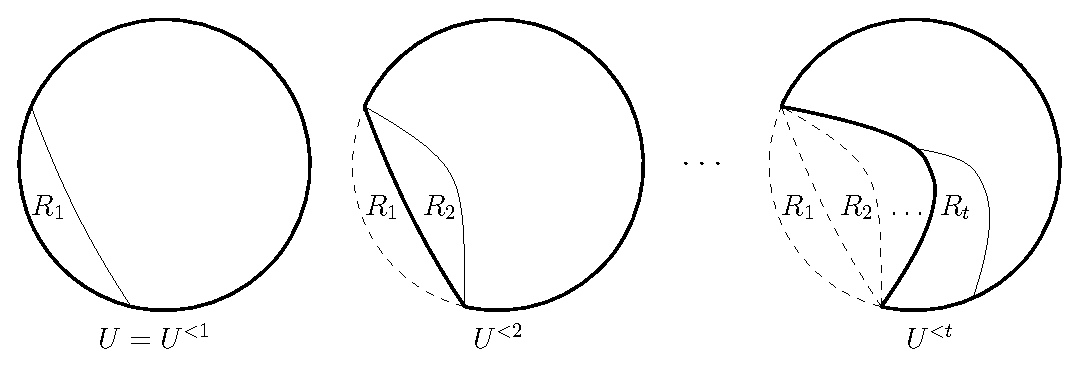
\includegraphics[scale=0.8]{nested_cuts.eps}
	\end{minipage}
	\caption{Sequence of nested cuts.}
	\label{fig:nested}
\end{figure}

\begin{lemma}[Properties of a sequence of nested cuts]
	\label{lem:seqbounds}
	Let $b, \phi \in (0,1)$ be such that $\phi \le b$, and $\delta \in (0,1]$. Fix a  cluster $U \subseteq V$, let $\theta \in \mathbb{R}_{\ge 0}$ be such that $\theta \le \frac{1}{5}\unvolc{U}{U}$, and let $R_1, \dots, R_t$ be a sequence of cuts \smash{$\emptyset \neq R_i \subsetneq U^{<i}$} where \smash{$ U^{<i} = U \setminus (\cup_{z =1}^{i-1} R_z)$} for all $i \in [t]$. If
	\begin{enumerate}
		\item \label{prec:sparse} for all $\emptyset \neq  X \subsetneq U$ with $\unspc{X}{U} < \delta \phi$ and $ \unvolc{X}{U} \le \unvolc{U \setminus X}{U}$ one has $\unvolc{X}{U}~<~\theta$,~and
		\item \label{prec:balsparse} for all $i \in [t]$ one has \smash{$\unspc{R_i}{U^{<i}} < \delta \phi$} and $ \unvolc{R_i}{U^{<i}} < \frac{1}{5}\unvolc{U}{U}$,
	\end{enumerate}
	then we have the following.
	\begin{enumerate}
		\item \label{part:1} For all $i \in [t]$, one has $\unspc{\cup_{z=1}^i R_z}{U} < \delta \phi$ and  $\unvolc{\cup_{z=1}^i R_z}{U} < \theta$.
		\item  \label{part:2b} For all $i \in [t]$, if there is $\theta^{\low} \in \mathbb{R}_{\ge 0}$ such that $\unvolc{R_i}{U^{<i}} \ge \theta^{\low}$ then one also has $\unvolc{R_i}{U} \ge \theta^{\low}-b\cdot \theta$.
		\item  \label{part:2c} Let $ U^{<t+1} = U \setminus (\cup_{z =1}^{t} R_z)$. If $\emptyset \neq R \subsetneq U^{<t+1}$ is a cut such that \smash{$\unspc{R}{U^{<t+1}} < \delta \phi$} and \smash{$\theta^{\low} \le \unvolc{R}{U^{<t+1}} \le \frac{5}{9}\unvolc{U^{<t+1}}{U^{<t+1}}$} for some $\theta^{\low} \le \frac{4}{9}\unvolc{U}{U}$, then \smash{$\unspc{R}{U} < \delta \phi \cdot \frac{\unvolc{U}{U}}{\theta^{\low}-b \cdot \theta}$} and $\theta^{\low}-b \cdot \theta \le \unvolc{R}{U} \le \frac{5}{9}\unvolc{U}{U}$.
	\end{enumerate}
\end{lemma}
 
 \noindent
 The end goal of part~\eqref{part:1} is to upper bound the number of edges crossing and the remaining volume when \cref{alg:trim} returns $(A,\top)$ and therefore \cref{alg:expdec} recurses on $U \setminus A$ only (see line~\eqref{enum:stoprec} in \cref{alg:expdec}). The idea is that in this case $U \setminus A$ corresponds to the union of nested cuts that are trimmed off by \cref{alg:trim}.
 
 Part~\eqref{part:2b} will be useful to bound the number of iterations that \cref{alg:trim} can take. In every iteration a cut is trimmed off, and from condition~\eqref{condition:baltrim} we know the volume of these cuts to be not too small in $U^{<i}$. From part~\eqref{part:2b} we then know these volumes to be not too small in $U$ either, and hence the number of such cuts cannot be too large, since they are disjoint.
 
  The end goal of part~\eqref{part:2c} is to upper bound the number of edges crossing and the remaining volume when \cref{alg:trim} returns $(R,\bot)$ and therefore \cref{alg:expdec} recurses on $R$ and $U \setminus R$ (see line~\eqref{enum:balrecurse} in \cref{alg:expdec}). The idea is that in this case, every cut trimmed off by \cref{alg:trim} is sparse and far from being balanced (because of condition~\eqref{enum:relaxouter} in \cref{alg:trim}), whereas the last one is both sparse and somewhat balanced (because of condition~\eqref{enum:relaxouter} in \cref{alg:trim}).
 \\~\\
 In the remainder of this section we prove the three parts of this lemma.
 \begin{proof}[Proof of \cref{lem:seqbounds}, part~\eqref{part:1}]
 	Intuitively, the union of a sequence of nested sparse and small cuts should be sparse and small too. We prove this by induction on $i \in [t]$. Denote for convenience~$\psi~=~\delta~\phi$.
 	
 	The base case for $i=1$ readily follows. Since $U^1 =U$, we have $\unspc{R_1}{U} < \psi$ and also $\unvolc{R_1}{U} < \frac{1}{5}\unvolc{U}{U}$ from precondition~\eqref{prec:balsparse}. Moreover,  by precondition~\eqref{prec:sparse}, there is no $\psi$-sparse cut $X$ with $\theta \le \unvolc{X}{U} < \frac{1}{2}\unvolc{U}{U}$. Hence, it must be the case that $\unvolc{R_1}{U} < \theta$.
 	
 	For the inductive step, take $i \in [t-1]$ and assume that $\unspc{\cup_{z=1}^i R_z}{U} < \psi$ and $\unvolc{\cup_{z=1}^i R_z}{U} < \theta$. We now apply Lemma~\ref{lem:relationsvol} with $S = U^{<i+1}$ and $T = R_{i+1}$. We can do so because $\unspc{S}{U} = \unspc{\cup_{z=1}^i R_z}{U} < \psi$, so the lemma gives
 	\begin{align*}
 		\unvolc{R_{i+1}}{U} \le \unvolc{R_{i+1}}{U^{<i+1}} \le \frac{1}{5}\unvolc{U}{U}  < \frac{1}{4}\unvolc{U}{U}\, .
 	\end{align*}
 	Combining this bound with the inductive hypothesis that $\unvolc{\cup_{z=1}^i R_z}{U} < \theta$, one has
 	\begin{equation*}
 		\unvolc{\cup_{z=1}^{i+1} R_z}{U} = \unvolc{\cup_{z=1}^i R_z}{U}+\unvolc{R_{i+1}}{U} < \theta+\unvolc{R_{i+1}}{U} < \frac{1}{5}\unvolc{U}{U}+ \frac{1}{4}\unvolc{U}{U}  < \frac{1}{2}\unvolc{U}{U} \, ,
 	\end{equation*}
 which rewrites as $\unvolc{T \cup (U \setminus S)}{U} < \frac{1}{2} \unvolc{U}{U}$ with  $S = U^{<i+1}$ and $T = R_{i+1}$. Also, from precondition~\eqref{prec:balsparse}, we have $\unspc{R_{i+1}}{U^{<i+1}} < \psi$, or in other words $\unspc{T}{S} < \psi$ with $S = U^{<i+1}$ and $T = R_{i+1}$. Then, the second part of Lemma~\ref{lem:relationsvol} gives $\unspc{\cup_{z=1}^{i+1} R_z}{U} < \psi$, so one part of the induction is proved. For the other part, we combine $\unspc{\cup_{z=1}^{i+1} R_z}{U} < \psi$ and $\unvolc{\cup_{z=1}^{i+1} R_z}{U} < \frac{1}{2}\unvolc{U}{U}$ with precondition~\eqref{prec:sparse}: since we assume there is no $\psi$-sparse cut in $G[U]^\circ$ with volume sandwiched between $\theta$ and $\frac{1}{2}\unvolc{U}{U}$, it must be the case that $\unvolc{\cup_{z=1}^{i+1} R_z}{U} < \theta$.
\end{proof}

 \begin{proof}[Proof of \cref{lem:seqbounds}, part~\eqref{part:2b}]
 	We prove this using part~\eqref{part:1} and \cref{lem:relationsvol}. The case of $i=1$ follows from the preconditions, since $U^1=U$. Let then $i =2, \dots, t$, and denote for convenience~$\psi~=~\delta~\phi$. Then, part~\eqref{part:1} gives that $\unspc{\cup_{z=1}^{i-1} R_z}{U} < \psi$. If we set $S=U^{<i}$ and $T=R_i$ we have $\unspc{S}{U} = \unspc{\cup_{z=1}^{i-1} R_z}{U} < \psi$, and can then apply \cref{lem:relationsvol} to get the lower bound
	\begin{align*}
		\unvolc{R_i}{U} & > \unvolc{R_i}{U^{<i}} - \delta b \cdot \unvolc{\cup_{z=1}^{i-1} R_z}{U} \\
		\text{since $\delta \le 1$} \quad & \ge  \unvolc{R_i}{U^{<i}} - b \cdot \unvolc{\cup_{z=1}^{i-1} R_z}{U} \, .
	\end{align*}
	Part~\eqref{part:1} also gives $\unvolc{\cup_{z=1}^{i-1} R_z}{U} < \theta $, and since we assume that $ \unvolc{R_i}{U^{<i}} \ge \theta^{\low}$, one concludes
		\begin{equation*}
		\unvolc{R_i}{U} > \unvolc{R_i}{U^{<i}} - b \cdot \unvolc{\cup_{z=1}^{i-1} R_z}{U}  \ge \theta^{\low} - b\cdot \theta \, .
	\end{equation*}
\end{proof}

 \begin{proof}[Proof of \cref{lem:seqbounds}, part~\eqref{part:2c}]
	We begin by analysing the volume $\unvolc{R}{U}$. Again, from part~\eqref{part:1} we have
	\begin{equation*}
		\unspc{\cup_{i=1}^{t} R_i}{U} < \delta \phi\, , \quad \unvolc{\cup_{i=1}^{t} R_i}{U} < \theta \,.
	\end{equation*}
	Setting $\psi = \delta \phi$, $S=U^{<t+1}$ and $T=R$,  we have $\unspc{S}{U} = \unspc{\cup_{z=1}^t R_z}{U} < \psi$, so we can apply \cref{lem:relationsvol} to yield
	\begin{equation} \label{eq:lbR}
		\unvolc{R}{U} > \unvolc{R}{U^{<t+1}} - b \cdot \unvolc{\cup_{i=1}^{t} R_i}{U} > \theta^{\low}-b \cdot \theta \, ,
	\end{equation}
	and
	\begin{equation}  \label{eq:ubR}
		\unvolc{R}{U} \le \unvolc{R_t}{U^{<t+1}} \le \frac{5}{9}\unvolc{U^{<t+1}}{U^{<t+1}} \, .
	\end{equation}
	We can once more apply Lemma~\ref{lem:relationsvol} with $S=T=U^{<t+1}$ (since again $\unspc{S}{U} = \unspc{\cup_{z=1}^t R_z}{U} < \psi$), so
	\begin{equation}
		 \label{eq:ubU}
		\unvolc{U^{<t+1}}{U^{<t+1}} \le \unvolc{U}{U} \, .
	\end{equation}
	We then have from~\eqref{eq:lbR},~\eqref{eq:ubR},~\eqref{eq:ubU}
	\begin{equation}
		\label{eq:sandwichR}
		 \theta^{\low}-b \cdot \theta \le \unvolc{R}{U} \le  \frac{5}{9}\unvolc{U^{<t+1}}{U^{<t+1}} \le  \frac{5}{9}\unvolc{U}{U} \, .
	\end{equation}
	Next we analyse the sparsity of $R$ by first upper-bounding the quantity $\uncut{R}{U}$:
	\begin{align}
		\uncut{R}{U} & \le {\uncut{R}{U^{<t+1}}+\uncut{(\cup_{i =1}^{t}R_i)}{U}} \\
		\text{since $\unspc{R}{U^{<t+1}} <\psi$ by assumption}\quad& < {\psi \cdot \unvolc{R}{U^{<t+1}}+\uncut{(\cup_{i =1}^{t}R_i)}{U}}\\
		\text{since $\unspc{\cup_{i =1}^{t}R_i}{U} <\psi$ from part~\eqref{part:1}} \quad & < {\psi \cdot \unvolc{R}{U^{<t+1}}+\psi \cdot \unvolc{\cup_{i =1}^{t}R_i}{U}} \\
		\text{since $\unvolc{R}{U} < \frac{5}{9}\unvolc{U}{U}$ from~\eqref{eq:sandwichR}} \quad& < {\psi \cdot  \frac{5}{9} \cdot \unvolc{U}{U}+\psi \cdot \unvolc{\cup_{i =1}^{t}R_i}{U}}\\
		\text{since $\unvolc{\cup_{i =1}^{t}R_i}{U}< \theta $ from  part~\eqref{part:1}}\quad & < \psi \cdot  \frac{5}{9} \cdot \unvolc{U}{U}+\psi \cdot \theta  \\
		\text{by assumption on $\theta$}\quad & < \psi \cdot {\unvolc{U}{U}} \, . \label{eq:ubcutR}
	\end{align}
On the other hand, the bounds in~\eqref{eq:sandwichR} yield
\begin{align}
	\min\{\unvolc{R}{U},\unvolc{U \setminus R}{U}\} & \ge 	\min\left\{ \theta^{\low}-b \cdot \theta, \frac{4}{9}\unvolc{U}{U}\right\} \\
	\text{since $\theta^{\low} \le \frac{4}{9} \unvolc{U}{U} $ by assumption} \quad & = \theta^{\low}-b \cdot \theta \, .  \label{eq:lbminvolR}
\end{align}
From the bound~\eqref{eq:ubcutR} and~\eqref{eq:lbminvolR} we finally conclude
\begin{equation*}
	\unspc{R}{U} = \frac{	\uncut{R}{U}}{\min\{\unvolc{R}{U},\unvolc{U \setminus R}{U}\}} < \frac{\psi \cdot {\unvolc{U}{U}}}{\theta^{\low}-b \cdot \theta} \, .
\end{equation*}
\end{proof}

\subsubsection{Relations between volume estimates}
\label{subsubsec:estim}
In this section we show how relations between volume estimates (such as the comparisons performed by \cref{alg:expdec} in line~\eqref{enum:balrecurse} and by \cref{alg:trim} in lines~\eqref{enum:relaxouter} and~\eqref{condition:baltrim}) translate to relations between the actual volumes of the corresponding cuts.

\begin{lemma}[Relations between volume estimates]
	\label{lem:algovols}
	Let $b, \phi, c \in (0,1)$ be such that $c \leq 1/4$ is a constant and $\phi \le b$. Fix a cluster $U \subseteq V$, and also let $H=(V,E',w)$ such that $H[U]^\circ \approx_c G[U]^\circ$, and let $\omega$ be a  $(\psi,\alpha',\lambda', c)$-BSCW of~$G[U]^\circ$ for some $\psi \in (0,\phi]$ and $\alpha',\lambda' \ge 1$. If $\omega = (R,\nu)$ for some $\emptyset \neq R \subsetneq U$ and $\nu \in \mathbb{R}_{>0}$, then for any $\rho,\tau \in [0,1]$ and $X \subseteq V$ we have
	\begin{enumerate}
		\item if $\nu \ge \rho \cdot \left(\wvolc{X}{X}\right)^\tau$, then $\unvolc{R}{U} \ge \rho/2 \cdot \left(\unvolc{X}{X}\right)^\tau$.
		\item if $\nu < \rho \cdot \left(\wvolc{X}{X}\right)^\tau$, then $\unvolc{R}{U} < 2\rho \cdot \left(\unvolc{X}{X}\right)^\tau$ and for every cut $\emptyset \neq  S \subsetneq U$ with $\unspc{S}{U} < \psi$ and $ \unvolc{S}{U} \le \unvolc{U \setminus S}{U}$ one has $\unvolc{S}{U} < 2\lambda' \rho \cdot \left(\unvolc{X}{X}\right)^\tau $.
	\end{enumerate}
\end{lemma}
\begin{proof}
	From property~\eqref{item:goodestimr} of the definition of BSCW (see \cref{def:bscw}), we know $(1-c)\unvolc{R}{U} \le \nu \le (1+c)\unvolc{R}{U} $, and from property~\eqref{item:balr} we know  that for every cut $\emptyset \neq  S \subsetneq U$ with $\unspc{S}{U} < \psi$ and $ \unvolc{S}{U} \le \unvolc{U \setminus S}{U}$ one has $\unvolc{S}{U} < \lambda'  \cdot \unvolc{R}{U}$.
	
	On the other hand, $(1-c)\unvolc{X}{X} \le \wvolc{X}{X} \le (1+c)\unvolc{X}{X}$ for any $X \subseteq V$. To see why, first note that $\wvolc{X}{X}=\wvol{X}+\frac{b-\phi}{\phi}\wbor{X}{X}=\wvol{X}+\frac{b-\phi}{\phi}\wcutg{X}$, and analogously \smash{$\unvolc{X}{X}=\vol(X)+\frac{b-\phi}{\phi}\uncutg{X}$}. Then, since $H[U]^\circ \approx_c G[U]^\circ$, we have the approximation guarantee for global cuts (see \cref{def:spars}): applying it to all singleton cuts in $X$ we can approximate $\vol(X)$, and applying it to $X$ we can approximate $\uncutg{X}$.
	
	From the above discussion it follows that for all $\rho,\tau \in [0,1]$ and $X \subseteq V$, $\nu \ge \rho \cdot \left(\wvolc{X}{X}\right)^\tau$ implies $\unvolc{R}{U} \ge \rho \frac{1-c}{1+c} \cdot \left(\unvolc{X}{X}\right)^\tau \ge \rho/2 \cdot \left(\unvolc{X}{X}\right)^\tau$, since $c \le 1/4$.  If instead $\nu < \rho \cdot \left(\wvolc{X}{X}\right)^\tau$, we have \smash{$\unvolc{R}{U} < \rho \frac{1+c}{1-c} \cdot \left(\unvolc{X}{X}\right)^\tau \le 2\rho \cdot \left(\unvolc{X}{X}\right)^\tau$}. Moreover, since by definition of $\omega$ one has $\unvolc{S}{U} < \lambda'  \cdot \unvolc{R}{U}$  for every cut $\emptyset \neq  S \subsetneq U$ with $\unspc{S}{U} < \psi$ and $ \unvolc{S}{U} \le \unvolc{U \setminus S}{U}$, we get $\unvolc{S}{U} < \lambda'  \cdot \unvolc{R}{U} \le \lambda' 2\rho \cdot \left(\unvolc{X}{X}\right)^\tau$ for any such $S$.
\end{proof}

\subsubsection{Bounding the number of iterations}
\label{subsubsec:iter}

\noindent
Combining the structural properties of nested cuts together with \cref{lem:algovols}, we can show the correctness of the algorithms. We begin by observing that whenever \cref{alg:trim} breaks the inner loop in line~\eqref{enum:break} we have $j \le k$. This ensures that restraining the outer loop to indices $j=1,\dots, k+1$ (see line~\eqref{enum:outerloop}) does not lead to undefined behaviour.

\begin{lemma}[\cref{alg:trim} does few outer loop iterations]
	\label{lem:boundouterloop}
	Let $b, \phi,c \in (0,1)$ such that $c \leq 1/30$ is a constant, $\phi < b$ and $b \le c$. Also let $C \ge 3$ be a constant, and let $\bsc$ be an $(\alpha,\lambda)$-BSCA where $\alpha \le \frac{1}{2b}$. If \cref{assump:sparsifiers2} holds, then if Algorithm~\ref{alg:trim} breaks in line~\eqref{enum:break} it is in some outer loop iteration $j$ with $j \le k$.
\end{lemma}
\begin{proof}
	We prove this by contradiction, so suppose the algorithm enters line~\eqref{enum:break} with $j=k+1$ for some inner loop iteration $h \ge 1$. Let $A$ be the value of the corresponding variable in \cref{alg:trim} at the beginning of inner loop iteration $h$ within outer loop iteration $k+1$. Also let $H=(V,E',w)$ be the graph gotten from line~\eqref{enum:freshsampletrim} in the same iteration. From the description of the algorithm, since it entered line~\eqref{enum:break}, the call $\bsc(H[A]^\circ, (1+{1}/{(2\log n)}) \cdot \phi_{k+1})$ from line~\eqref{enum:trimcallbalsparse} has returned a BSCW of the form $(R,\nu)$ such that \smash{$\nu< \frac{1}{C\lambda}(\wvolc{U}{U})^{1-(k+1-1)/k}=\frac{1}{C\lambda}(\wvolc{U}{U})^0$}. Moreover, since we have $c \le 1/30$, $\phi < b$, $b \le c$, $\alpha \le \frac{1}{2b}$,  and $H[A] \approx_{\delta_{k+1}} G[A]$ (from \cref{assump:sparsifiers2}), \cref{lem:reduction} ensures that $(R,\nu)$ is a \smash{$(\phi_j,(1+\frac{1}{\log n})\alpha,(1+c)\lambda, c)$}-BSCW of~$G[A]^\circ$ (see \cref{rmk:bsctrim}).
	
	We now want to use Lemma~\ref{lem:algovols} with $\psi = \phi_{k+1}$, $ \alpha'=(1+\frac{1}{\log n})\alpha$, $\lambda' =(1+c)\lambda$, $\rho= \frac{1}{C\lambda}$, $\tau=0$, and $X=U$. These parameters verify the conditions for applying \cref{lem:algovols} to $(R,\nu)$ on $G[A]^\circ$: $c \le 1/30 \le 1/4$, $\psi = \phi_{k+1} \le \phi$ (by definition of $\phi_{k+1}$ in the algorithm), $\alpha',\lambda' \ge 1$, $\rho \le 1$, $\tau \in [0,1]$, $H[A] \approx_{c} G[A]$ (since $H[A] \approx_{\delta_{k+1}} G[A]$ and $\delta_{k+1} \le c$), and  hence $(R,\nu)$ is a \smash{$(\phi_j,(1+\frac{1}{\log n})\alpha,(1+c)\lambda, c)$}-BSCW of~$G[A]^\circ$. Then \cref{lem:algovols} gives
	\begin{equation*}
		\unvolc{R}{A} < 2 \rho (\unvolc{U}{U})^\tau = \frac{2}{C\lambda} < 1 \, ,
	\end{equation*}
	which in particular implies $R=\emptyset$. However, this contradicts the fact that $(R,\nu)$ is a BSCW of~$G[A]^\circ$ (see \cref{def:bscw}).
\end{proof}

\noindent
Next, we show that \cref{alg:trim} verifies the preconditions~\eqref{prec:sparse} and~\eqref{prec:balsparse} of \cref{lem:seqbounds}. Specifically, if \cref{alg:expdec} calls \cref{alg:trim}, there cannot be sparse and balanced cuts in $U$, and also every cut trimmed by \cref{alg:trim} is sparse and small in volume. This will later allow us to apply \cref{lem:seqbounds} for bounding the number of inner loop iterations (and also for bounding the recursion depth, in the next section).

\begin{lemma}[\cref{alg:trim} makes a sequence of nested sparse small cuts]
	\label{lem:boundsequencetrim}
	Let $b, \phi,c \in (0,1)$ such that $c \leq 1/30$ is a constant, $\phi < b$ and $b \le c$. Also let $C \ge 11$ be a constant, and let $\bsc$ be an $(\alpha,\lambda)$-BSCA where $\alpha \le \frac{1}{2b}$. Consider an execution of \cref{alg:trim} called from \cref{alg:expdec} on input cluster $U \subseteq V$. Also let $R_1,\dots,R_q \subseteq U$ be the sequence of $q$ cuts trimmed in line~\eqref{enum:trim} by \cref{alg:trim}, and let $U^{<i}=U \setminus (\cup_{z-1}^{i-1}R_z)$. If \cref{assump:sparsifiers1} and \cref{assump:sparsifiers2} hold, then
	\begin{enumerate}
		\item \label{satprec:sparse} for all \smash{$\emptyset \neq  S  \subsetneq U$} with \smash{$\unspc{S}{U} < \phi$, $ \unvolc{S}{U} \le \unvolc{U \setminus S}{U}$}, one has \smash{$\unvolc{S}{U}<\frac{3}{C}\unvolc{U}{U}$},
		\item \label{satprec:balsparse} for all $i \in [q]$ one has \smash{$\unspc{R_i}{U^{<i}} < \phi$} and $ \unvolc{R_i}{U^{<i}} < \frac{1}{5}\unvolc{U}{U}$.
	\end{enumerate}
\end{lemma}
\begin{proof}
	From the description of Algorithms~\ref{alg:expdec} and~\ref{alg:trim}, we see that Algorithm~\ref{alg:trim} starts only if line~\eqref{enum:balsparsecall} of \cref{alg:expdec} returns a BSCW $\omega=(R,\nu)$ such that $\nu < \frac{1}{C \lambda}\wvolc{U}{U}$, as per line~\eqref{enum:gotrim} (otherwise, \cref{alg:expdec} would not call \cref{alg:trim}). Now we want to apply \cref{lem:reduction} to $\omega$. Because we have $c\le 1/30$, $\phi < b$, $b \le c$, $\delta=c^2 b/\log n $, $\alpha \le \frac{1}{2b}$ and $H[U] \approx_{\delta} G[U]$ from \cref{assump:sparsifiers1}, all the preconditions of \cref{lem:reduction} are met for us to apply it to the call $\bsc(H[U]^\circ, (1+\frac{1}{2\log n}) \cdot \phi)$ from line~\eqref{enum:balsparsecall} of \cref{alg:expdec}: hence, $\omega$ is a  \smash{$(\phi,(1+\frac{1}{\log n})\alpha,(1+c)\lambda, c)$}-BSCW of~$G[U]^\circ$. Since we observed just above that $\omega$ is of the form $(R,\nu)$ and \smash{$\nu < \frac{1}{C \lambda}\wvolc{U}{U}$}, we now use \cref{lem:algovols} with parameters $\psi=\phi$, \smash{$ \alpha'=(1+\frac{1}{\log n})\alpha$}, $\lambda' =(1+c)\lambda$, \smash{$\rho = \frac{1}{C\lambda}$}, $\tau=1$, and $X=U$. These parameters verify the requirement of \cref{lem:algovols} since we have $ c\le 1/30 \le 1/4$, $H[U] \approx_{c} G[U]$ (from \cref{assump:sparsifiers1}, since $\delta \le c$), $\psi \le \phi$, $\alpha',\lambda' \ge 1$, $\rho,\tau \le 1$, and  $(R,\nu)$ is a \smash{$(\phi,(1+\frac{1}{\log n})\alpha,(1+c)\lambda,c)$}-BSCW of~$G[U]^\circ$. Then we get that for every cut $\emptyset \neq  S \subsetneq U$ with $\unspc{S}{U} < \phi$ and $ \unvolc{S}{U} \le \unvolc{U \setminus S}{U}$ one has
	\begin{equation*}
		\unvolc{S}{U} < 2\lambda' \rho \cdot \unvolc{U}{U} = \frac{2(1+c)\lambda}{C\lambda}  \unvolc{U}{U} \leq \frac{3}{C} \cdot \unvolc{U}{U} \, .
	\end{equation*}
	This gives part~\eqref{satprec:sparse}.
	
	For all $i \in [q]$, denote by $j(i) \in [k+1]$ the outer loop iteration of \cref{alg:trim} where $R_i$ was trimmed, and also let $U^{<i}=U \setminus (\cup_{z=1}^{i-1} R_z)$ (i.e., at the beginning of the iteration where $R_i$ has been trimmed we had $A = U^{<i}$). Then, from the description of the algorithm we know that $R_i$ was paired with a value $\nu_{R_i}$ such that $(R_i,\nu_{R_i})$ was the result of $\bsc(H[U^{<i}]^\circ, (1+\frac{1}{2\log n}) \cdot \phi_{j(i)-1})$, where $H=(V,E',w)$ verifies \smash{$H[U^{<i}] \approx_{\delta_{j(i)}} G[U^{<i}] $} because of \cref{assump:sparsifiers2}. As we have $ c\le 1/30$, $\phi < b$, $b \le c$, \smash{$\alpha \le \frac{1}{2b}$}, \cref{lem:reduction} ensures that the pair $(R_i,\nu_{R_i})$ is a \smash{$(\phi_{j(i)},(1+\frac{1}{\log n})\alpha,(1+c)\lambda,c)$}-BSCW of~$G[U^{<i}]^\circ$ for all $i \in [q]$ (see \cref{rmk:bsctrim}).  From the description of the algorithm  we also know that $\nu_{R_i}$ must also not satisfy condition~\eqref{enum:relaxouter}, as otherwise \cref{alg:trim} would have returned, so $\nu_{R_i} < \frac{1}{C \lambda}\wvolc{U}{U}$ for all $i \in [q]$. For each $i \in [q]$, we now use \cref{lem:algovols} with parameters $\psi=\phi_{j(i)}$, \smash{$ \alpha'=(1+\frac{1}{\log n})\alpha$}, $\lambda' =(1+c)\lambda$, $\rho = \frac{1}{C\lambda}$, $\tau=1$, and $X=U$. These parameters verify the requirement for applying \cref{lem:algovols} to $(R_i,\nu_{R_i})$ in $G[U^{<i}]$: $ c\le 1/30 \le 1/4$, $H[U^{<i}] \approx_{c} G[U^{<i}]$ (from \cref{assump:sparsifiers2} and $\delta_{j(i)} \le c$), $\psi=\phi_{j(i)}\le \phi$, $\alpha',\lambda' \ge 1$, $\rho,\tau \le 1$, and $(R_i,\nu_{R_i})$ is a \smash{$(\phi_{j(i)},(1+\frac{1}{\log n})\alpha,(1+c)\lambda, c)$}-BSCW of~$G[U^{<i}]^\circ$. Then, for all $i \in [q]$ \cref{lem:algovols} gives
	\begin{equation}
		\label{eqclaim:bal}
		\unvolc{R_i}{U^{<i}} < \frac{2}{C\lambda}\unvolc{U}{U} < \frac{1}{5}\unvolc{U}{U}\, ,
	\end{equation}
	since $C \ge 11$.
	Furthermore, because every $(R_i,\nu_{R_i})$ is a \smash{$(\phi_{j(i)},(1+\frac{1}{\log n})\alpha,(1+c)\lambda, c)$}-BSCW of~$G[U^{<i}]^\circ$, we have by \cref{def:bscw}
	\begin{equation}
		\label{eqclaim:sparse}
		\unspc{R_i}{U^{<i}} < \left(1+\frac{1}{ \log n}\right) \alpha \phi_{j(i)} = \left(1+\frac{1}{ \log n}\right) \alpha \frac{\phi}{\left( \left(1+\frac{1}{ \log n}\right) \alpha\right)^{j(i)}}  \le \phi \, ,
	\end{equation}
	since $j(i) \ge 1$. The bounds in~\eqref{eqclaim:bal} and~\eqref{eqclaim:sparse} give part~\eqref{prec:balsparse}.
\end{proof}

\noindent
Finally, we argue that \cref{alg:trim} goes through few inner loop iterations within each outer loop iteration. The idea for this is that we can upper bound the total volume trimmed in line~\eqref{enum:trim}, but we can also lower bound the volume of each individual cut.

\begin{lemma}[\cref{alg:trim} does few inner loop iterations]
	\label{lem:boundinnerloop}
	Let $b, \phi,c \in (0,1)$ such that $c \leq 1/30$ is a constant, $\phi < b$ and $b \le c$. Also let $C \ge 31$ be a constant, let $\bsc$ be an $(\alpha,\lambda)$-BSCA where $\alpha \le \frac{1}{2b}$ and $\lambda \le \frac{c}{2b}$, and let $k$ be an integer such that \smash{$k \ge \log \frac{n^2}{\phi}/\log \frac{c}{\lambda \cdot b}$}. If \cref{assump:sparsifiers1} and \cref{assump:sparsifiers2} hold, then \cref{alg:trim} goes through at most $1/{b}$ inner loop iterations within each outer loop iteration.
\end{lemma}
\begin{proof}
	Let $U$ be the input cluster of \cref{alg:trim}. Fix hereafter an outer loop iteration $j=1,\dots, k+1$, and let $A$ be the value of the corresponding variable of the algorithm at the beginning of the $j$-th outer loop iteration. Because line~\eqref{enum:trim} of \cref{alg:trim} removes a non-empty cut from $A$ at every inner loop iteration, there are finitely many iterations. Denote then by $t$ the number of inner loop iterations for outer loop iteration $j$. Then, for every  inner loop iteration $h\in [t]$ define $A^{<h}$ to be the value of variable $A$ at the beginning of inner loop iteration $h$.
	
	Since \cref{assump:sparsifiers2} holds,  we also know that to every inner loop iteration $h \in [t]$ corresponds a graph $H=(V,E',w)$ from line~\eqref{enum:freshsampletrim} which satisfies $H[A^{<h}] \approx_{\delta_j} G[A^{<h}]$. As we have $c \le 1/30$, $\phi < b$, $b \le c$, $\alpha \le \frac{1}{2b}$,  and $H[A^{<h}] \approx_{\delta_j} G[A^{<h}]$, \cref{lem:reduction} ensures that calling $\bsc(H[A^{<h}]^\circ, (1+\frac{1}{2\log n}) \cdot \phi_j)$ gives a \smash{$(\phi_j,(1+\frac{1}{\log n})\alpha,(1+c)\lambda, c)$}-BSCW of~$G[A^{<h}]^\circ$ in line~\eqref{enum:trimcallbalsparse} of \cref{alg:trim} (see \cref{rmk:bsctrim}). Moreover, from the description of the algorithm, it must be the case that the BSCW obtained is of the form $(R_h,\nu_h)$ for all $h \in [t-1]$, where $\emptyset \neq R_h \subsetneq A^{<h}$ and $\nu_h \in \mathbb{R}_{> 0}$. One can then see that for every $h \in [t]$ we have $A^{<h}=A \setminus (\cup_{z=1}^{h-1}R_z)$, and because of conditions~\eqref{enum:relaxouter} and~\eqref{condition:baltrim} we have that for every $h \in [t-1]$ the following holds:
	\begin{equation*}
		\frac{1}{C\lambda}\left(\wvolc{U}{U}\right)^{1-(j-1)/k} \le \nu_h < \frac{1}{C\lambda}\wvolc{U}{U} \, .
	\end{equation*}
	We now want to translate the above bounds to $\unvolc{R_h}{A^{<h}}$ using \cref{lem:algovols}. To do so, note that $H[A^{<h}] \approx_{\delta_j} G[A^{<h}]$ in particular implies $H[A^{<h}] \approx_{c} G[A^{<h}]$ (since we have defined $\delta_j=c^2 b_j/\log n \le c$), and as discussed before we know that
	\begin{equation}
		\label{eq:bscw}
		\text{$(R_h,\nu_h)$ is a $\left(\phi_j,\left(1+\frac{1}{\log n}\right)\alpha,(1+c)\lambda,c\right)$-BSCW of~$G[A^{<h}]^\circ$}
	\end{equation}
	Let us then set $\psi=\phi_j$, $ \alpha'=(1+\frac{1}{\log n})\alpha$, $\lambda' =(1+c)\lambda$, $\rho = \frac{1}{C\lambda}$, $\tau$ being either $1-(j-1)/k$ (for the lower bound) or $1$ (for the upper bound), and $X=U$. These parameters verify the conditions for applying \cref{lem:algovols} to $(R_h,\nu_h)$ on $G[A^{<h}]^\circ$: $c \le 1/30 \le 1/4$, $\psi =\phi_j\le \phi$, $\alpha',\lambda' \ge 1$, $\rho \le 1$, both values of $\tau$ are bounded by $1$ (this is because $j \le k+1$), $H[A^{<h}] \approx_{c} G[A^{<h}]$ (since from \cref{assump:sparsifiers2} we have \smash{$H[A^{<h}] \approx_{\delta_j} G[A^{<h}]$}), and $(R_h,\nu_h)$ is a $(\phi_j,(1+\frac{1}{\log n})\alpha,(1+c)\lambda,c)$-BSCW of \smash{$G[A^{<h}]^\circ$} (see~\eqref{eq:bscw}). Then \cref{lem:algovols} gives
	\begin{equation}
		\label{sandwich:actual}
	\frac{1}{2C\lambda}\left(\unvolc{U}{U}\right)^{1-(j-1)/k} \le \unvolc{R_h}{A^{<h}} <\frac{2}{C\lambda}\unvolc{U}{U} \, ,
	\end{equation}
	where the lower bound is obtained with $\tau=1-(j-1)/k$ and the upper bound with $\tau=1$. The application of \cref{lem:algovols} with $\tau=1$ also gives that for every cut $\emptyset \neq  S \subsetneq A^{<h}$ with $\unspc{S}{A^{<h}} < \phi_j$ and $ \unvolc{S}{A^{<h}} \le \unvolc{A^{<h}\setminus S}{A^{<h}}$ one has
	\begin{equation}
		\label{eq:absolbal}
		\unvolc{S}{A^{<h}} < 2\lambda' \rho \cdot \unvolc{U}{U} = \frac{2(1+c)\lambda}{C\lambda}  \unvolc{U}{U} \le \frac{3}{C} \cdot \unvolc{U}{U} \, .
	\end{equation}
	We consider now the case of $j=1$ and $2 \le j \le k+1$ separately.
	
	\paragraph{Case $j=1$.} In this case $A$ is identical to the input cluster $U$.	We then want to apply Lemma~\ref{lem:seqbounds} with $\delta=1$ and $\theta = \frac{3}{C}\unvolc{U}{U}$ to the sequence of cuts $R_1,R_2, \dots, R_{t-1}$ in the cluster~$U$. Let for convenience $U^i = U \setminus (\cup_{z =1}^{i-1} R_z)$ for all $i \in [t]$.
	
	First note that this value of $\theta$ meets the requirement of \cref{lem:seqbounds} that $\theta< \frac{1}{5}\unvolc{U}{U}$, since $C \ge 16$. Secondly, our set of assumptions matches that of \cref{lem:boundsequencetrim}, so we get that for all \smash{$\emptyset \neq  S  \subsetneq U$} with \smash{$\unspc{S}{U} < \phi$, $ \unvolc{S}{U} \le \unvolc{U \setminus S}{U}$}, one has \smash{$\unvolc{S}{U}<\frac{3}{C}\unvolc{U}{U}$}, and for all $i \in [q]$ one has \smash{$\unspc{R_i}{U^{<i}} < \phi$} and $ \unvolc{R_i}{U^{<i}} < \frac{1}{5}\unvolc{U}{U}$. These facts match preconditions~~\eqref{prec:sparse} and~\eqref{prec:balsparse} of \cref{lem:seqbounds} for $\delta$ and $\theta$ as we set them above.
	
	Part~\eqref{part:1} of \cref{lem:seqbounds} then upper-bounds the total volume of the sequence as
	\begin{equation}
		\label{eq:totalubjone}
		\unvolc{\cup_{h=1}^{t-1} R_h}{U} < \frac{3}{C}\unvolc{U}{U} \, .
	\end{equation}
	Since the lower bound of~\eqref{eq:bscw} with $j=1$ means that $ \unvolc{R_h}{U^{<h}} \ge \frac{1}{2C\lambda}\unvolc{U}{U}$ for all $h \in [t-1]$, using part~\eqref{part:2b} of \cref{lem:seqbounds} with $\theta^{\low} =\frac{1}{2C\lambda}\unvolc{U}{U}$ we further get
		\begin{equation}
		\label{eq:indivlbjone}
		\unvolc{R_h}{U} \ge \frac{1}{2C\lambda}\unvolc{U}{U} - b\cdot \frac{3}{C}\unvolc{U}{U}  \ge  \frac{1}{3C\lambda}\unvolc{U}{U} \quad \text{ for all $h \in [t-1]$}\, ,
	\end{equation}
since  $\lambda \le \frac{1}{18b}$.
	Therefore, taking the ratio of the cumulative upper bound in~\eqref{eq:totalubjone} and the individual lower bounds from~\eqref{eq:indivlbjone}, we conclude that $t-1$ cannot exceed
	\begin{equation*}
		\frac{\unvolc{\cup_{h=1}^{t-1} R_h}{U}}{\min_{h \in [t-1]}\unvolc{R_h}{U}} \le \frac{\frac{3}{C}\unvolc{U}{U}}{\frac{1}{3C\lambda}\unvolc{U}{U}} \le 9 \lambda \, .
	\end{equation*}
Thus, the number of inner loop iterations for $j=1$ is at most $9\lambda +1 \le \frac{1}{2b}+1 \le 1/b$.
	
	\paragraph{Case $2 \le j \le k+1$.} The approach is analogous to the first iteration, except that we use the bounds from \cref{lem:seqbounds} on the sequence $R_1,\dots,R_{t-1}$ in the cluster $A$ (for $j=1$ we applied the lemma to the cluster $U$). We remark that, in this case, $A$ can also be seen as the value of the corresponding variable of \cref{alg:trim} at the very end of outer loop iteration $j-1$.
	
	Consider the call $\bsc(H[A]^\circ, (1+\frac{1}{2\log n}) \cdot \phi_{j-1})$ to $\bsc$ in the last inner loop iteration within outer loop iteration $j-1$, where $H=(V,E',w)$ is accordingly the graph obtained from line~\eqref{enum:freshsampletrim} at the last inner loop iteration within outer loop iteration~${j-1}$. Since \cref{assump:sparsifiers2} holds,  we know that the graph $H$ satisfies \smash{$H[A] \approx_{\delta_{j-1}} G[A]$}. As we have $c \le 1/30$, $\phi < b$, $b \le c$, $\alpha \le \frac{1}{2b}$,  and \smash{$H[A] \approx_{\delta_{j-1}} G[A]$}, \cref{lem:reduction} ensures that the call \smash{$\bsc(H[A]^\circ, (1+\frac{1}{2\log n}) \cdot \phi_{j-1})$} gives a \smash{$(\phi_{j-1},(1+\frac{1}{\log n})\alpha,(1+c)\lambda,c)$}-BSCW $\omega$ of $G[A]^\circ$ (see \cref{rmk:bsctrim}). On the other hand, from the description of the algorithm we know that iteration $j$ starts only if this $\omega$ is of the form $(R,\nu)$ with $\nu < \frac{1}{C \lambda}(\wvolc{U}{U})^{1-(j-2)/k}$ (due to condition~\eqref{condition:baltrim}). We now use \cref{lem:algovols} with parameters $\psi=\phi_{j-1}$, \smash{$ \alpha'=(1+\frac{1}{\log n})\alpha$}, $\lambda' =(1+c)\lambda$, $\rho = \frac{1}{C\lambda}$, $\tau=1-(j-2)/k$, and $X=U$. These parameters verify the requirement of \cref{lem:algovols} since we have $ c\le 1/30 \le 1/4$, $H[A] \approx_{c} G[A]$ (from \cref{assump:sparsifiers2} and $\delta_{j-1} \le c$), $\psi=\phi_{j-1}\le \phi$, $\alpha',\lambda' \ge 1$, $\rho,\tau \le 1$, and $(R,\nu)$ is a \smash{$(\phi_{j-1},(1+\frac{1}{\log n})\alpha,(1+c),c\lambda)$}-BSCW of~$G[A]^\circ$. Then we get that for every cut $\emptyset \neq  S \subsetneq A$ with $\unspc{S}{A} < \phi_{j-1}$ and $ \unvolc{S}{A} \le \unvolc{A \setminus S}{A}$ one has
	\begin{equation}
		\label{eq:generalcasenobsc}
		\unvolc{S}{A} < 2\lambda' \rho \left(\unvolc{U}{U}\right)^\tau =  \frac{2(1+c)\lambda}{C\lambda} \left( \unvolc{U}{U}\right)^{1-(j-2)/k} \le \frac{3}{C} \cdot \left(\unvolc{U}{U}\right)^{1-(j-2)/k} \, .
	\end{equation}
	This is still not enough to apply \cref{lem:seqbounds} to cluster $A$: the bound in~\eqref{sandwich:actual} bounds the volumes of nested cuts $R_h$ in $A^{<h}$ by $\frac{2}{C\lambda}\unvolc{U}{U}$, but applying \cref{lem:seqbounds} demands an upper bound of $\frac{1}{5}\unvolc{A}{A}$ on the volumes of cuts $R_h$ in $A^{<h}$. Hence, we first show the volume of $U$ to be not much larger than that of $A$.
	
	\begin{claim}
		\label{claim:voluvola}
		We have $\unvolc{U}{U} \le 2 \unvolc{A}{A}$.
	\end{claim}
	\begin{proof}
		If $A=U$ the statement is trivial. Otherwise, we know there must have been a sequence of nested cuts $S_1,\dots,S_r \subseteq U$ that \cref{alg:trim} trimmed off from $U$ in line~\eqref{enum:trim} so that $A=U \setminus (\cup_{i \in [r]} S_i)$. We then want to apply Lemma~\ref{lem:seqbounds} to the sequence of cuts $S_1,S_2, \dots, S_r$ in the cluster~$U$ with $\delta=1$ and $\theta = \frac{3}{C}\unvolc{U}{U}$. Let for convenience $U^{<i} = U \setminus (\cup_{z =1}^{i-1} S_z)$ for all $i \in [r+1]$.
		
		First note that this value of $\theta$ meets the requirement of \cref{lem:seqbounds} that $\theta< \frac{1}{5}\unvolc{U}{U}$, since $C \ge 16$. Secondly, our set of assumptions matches that of \cref{lem:boundsequencetrim}, so we get that for all \smash{$\emptyset \neq  S  \subsetneq U$} with \smash{$\unspc{S}{U} < \phi$, $ \unvolc{S}{U} \le \unvolc{U \setminus S}{U}$}, one has \smash{$\unvolc{S}{U}<\frac{3}{C}\unvolc{U}{U}$}, and for all $i \in [r]$ one has \smash{$\unspc{S_i}{U^{<i} } < \phi$} and $ \unvolc{S_i}{U^{<i}} < \frac{1}{5}\unvolc{U}{U}$ (the latter follows because part~\eqref{satprec:balsparse} of \cref{lem:boundsequencetrim} bounds the sparsity and volume of every cut in the entire sequence of cuts trimmed by the algorithm, and $S_1,\dots,S_r$ is a prefix of the entire sequence). These facts match preconditions~~\eqref{prec:sparse} and~\eqref{prec:balsparse} of \cref{lem:seqbounds} for $\delta$ and $\theta$ as set above. Part~\eqref{part:1} of \cref{lem:seqbounds} then upper-bounds the total volume of the sequence as
		\begin{equation}
			\label{bound:claim}
			\unvolc{\cup_{i=1}^{r} S_i}{U} < \frac{3}{C}\unvolc{U}{U} \, .
		\end{equation}
		To conclude it is sufficient to notice
		\begin{align*}
			\unvolc{U}{U} & = \unvolc{A}{U}+\unvolc{U \setminus A}{U}\\
			& = \unvolc{A}{U}+\unvolc{\cup_{i =1}^r S_i}{U} \\
			\text{$\unvolc{A}{A}$ cannot have less self-loops than $\unvolc{A}{U}$}\quad& \le \unvolc{A}{A}+\unvolc{\cup_{i =1}^r S_i}{U} \\
			\text{by~\eqref{bound:claim}}\quad & < \unvolc{A}{A}+\frac{3}{C}\unvolc{U}{U} \, ,
		\end{align*}
	and the claim follows since $C \ge 6$.
	\end{proof}
	
	\noindent
	By \cref{claim:voluvola} and~\eqref{sandwich:actual}, we have that for every $h \in [t-1]$
	\begin{equation}
		\label{eq:ubwrta}
		\unvolc{R_h}{A^{<h}} < \frac{2}{C\lambda}\unvolc{U}{U} \le \frac{4}{C\lambda}\unvolc{A}{A} < \frac{1}{5}\unvolc{A}{A} \, ,
	\end{equation}
	since $C \ge 21$. Furthermore, because every $(R_h,\nu_h)$ is a $(\phi_j,(1+\frac{1}{\log n})\alpha,(1+c)\lambda,c)$-BSCW of~\smash{$G[A^{<h}]^\circ$}, we have
	\begin{equation}
		\label{eq:sparse}
		\unspc{R_h}{A^{<h}} < \left(1+\frac{1}{ \log n}\right) \alpha \phi_{j} = \left(1+\frac{1}{ \log n}\right) \alpha \frac{\phi}{\left( \left(1+\frac{1}{ \log n}\right) \alpha\right)^{j}}  \le \phi_{j-1} \, .
	\end{equation}
	We are now in shape to apply Lemma~\ref{lem:seqbounds} to the sequence of cuts $R_1,R_2, \dots, R_{t+1}$ in the cluster~$A$. Specifically, we do this with $\delta=\phi_{j-1}/\phi$ and $\theta = \frac{3}{C}(\unvolc{U}{U})^{1-(j-2)/k}$. First observe that $\delta \le 1$ (by definition of $\phi_{j-1}$) and $ \theta \le  \frac{3}{C}\unvolc{U}{U} \le \frac{1}{5}\unvolc{A}{A}$ (again by \cref{claim:voluvola} and $C \ge 31$), as demanded by \cref{lem:seqbounds}. For these parameters, one can see that precondition~\eqref{prec:balsparse} is given by~\eqref{eq:ubwrta} and~\eqref{eq:sparse}. Precondition~\eqref{prec:sparse} is instead given by~\eqref{eq:generalcasenobsc}. Part~\eqref{part:1} of \cref{lem:seqbounds} then upper-bounds the total volume of the sequence as
	\begin{equation}
		\label{eq:ubgeneraliter}
		\unvolc{\cup_{h=1}^{t-1} R_h}{A} < \theta =  \frac{3}{C}\left(\unvolc{U}{U}\right)^{1-(j-2)/k} \, .
	\end{equation}
	We are left with lower bounding the volume of each individual cut. We do this with part~\eqref{part:2b} of \cref{lem:seqbounds} with $\theta^{\low} = \frac{1}{2C\lambda}(\unvolc{U}{U})^{1-(j-1)/k}$, which meets the requirement that $	\unvolc{R_h}{A} \ge \theta^{\low}$ thanks to the bound in~\eqref{sandwich:actual}. Part~\eqref{part:2b} of \cref{lem:seqbounds} then gives that for all $h \in [t-1]$
	\begin{align}
			\label{eq:lbgeneraliter}
		\unvolc{R_h}{A} \ge \theta^{\low} - b \cdot \theta = \frac{1}{2C\lambda}\left(\unvolc{U}{U}\right)^{1-(j-1)/k} - b \cdot  \frac{3}{C}\left(\unvolc{U}{U}\right)^{1-(j-2)/k}\, .
	\end{align}
	Therefore, taking the ratio of the upper bound on the total volume from~\eqref{eq:ubgeneraliter} and the lower bound on the volume of each individual cut from~\eqref{eq:lbgeneraliter}, we conclude that $t-1$ is at most
	\begin{align*}
		\frac{\unvolc{\cup_{h=1}^{t-1} R_h}{A}}{\min_{h \in [t-1]} \unvolc{R_h}{A}} & \le
		\frac{\frac{3}{C}\left(\unvolc{U}{U}\right)^{1-(j-2)/k}}{\frac{1}{2C\lambda}\left(\unvolc{U}{U}\right)^{1-(j-1)/k} - b \cdot \frac{3}{C}\left(\unvolc{U}{U}\right)^{1-(j-2)/k}} \\
		& = \frac{\frac{3}{C}\left(\unvolc{U}{U}\right)^{1/k}}{\frac{1}{2C\lambda} - b \cdot \frac{3}{C}\left(\unvolc{U}{U}\right)^{1/k}} \, .
	\end{align*}
	Next, we observe that $\unvolc{U}{U} \le \vol(V)\cdot b/\phi \le \vol(V)/{\phi} \le n^2/\phi$ (since in the worst case we over-count every edge in $G$ as a self-loop in $G[U]^{\circ}$ and  at most $b/\phi$ times). Then, using that \smash{$k \ge \log (\frac{n^2}{\phi}) / \log (\frac{c}{\lambda \cdot b})$}, it holds that \smash{$\left(\unvolc{U}{U}\right)^{1/k} \leq \frac{c}{\lambda \cdot b}$}. Now we can upper-bound the above as
	\begin{align*}
		\frac{\frac{3}{C}\left(\unvolc{U}{U}\right)^{1/k}}{\frac{1}{2C\lambda} - b \cdot \frac{3}{C}\left(\unvolc{U}{U}\right)^{1/k}}  \le \frac{\frac{3}{C}\left(\unvolc{U}{U}\right)^{1/k}}{\frac{1}{2C\lambda} - b \cdot \frac{3}{C}\frac{c}{\lambda \cdot b}} \le \frac{\frac{3}{C} \cdot \left(\frac{n^2}{\phi}\right)^{1/k}}{\frac{1}{5C \lambda} } \le \frac{\frac{3}{C} \cdot \frac{c}{\lambda \cdot b}}{\frac{1}{5C \lambda}} = 15 \frac{c}{b}\, ,
	\end{align*}
	since $c \le \frac{1}{30}$.	Hence, the number of inner loop iterations for $2 \le j \le k+1$ is at most $ \frac{15c}{b} +1\le \frac{1}{b}$.
\end{proof}

\subsubsection{Bounding the recursion depth}
\label{subsubsec:depth}
\noindent
From the description of the algorithms one can see that we recurse on both sides of a cut (in line~\eqref{rec:twosides} of \cref{alg:expdec}) only when the conditions~\eqref{enum:balrecurse} in \cref{alg:expdec} and~\eqref{enum:relaxouter} in \cref{alg:trim} suggest that the cut is balanced, so as to maintain the recursion depth small. When instead \cref{alg:expdec} recurses on one side only, in line~\eqref{rec:onside}, we can use the properties of nested cuts to upper bound the volume of the recursed side. To control the number of self-loops that we add after each recursion, we also want to ensure that we recurse on sparse cuts only.

\begin{lemma}[\cref{alg:expdec} recurses on balanced sparse cuts]
	\label{lem:recursioncut}
	Let $b, \phi,c \in (0,1)$ such that $c \le 1/30$ is a constant, $\phi < b$, $b \le c$. Also  let $C \ge 16$ be a constant, and let $\bsc$ be an $(\alpha,\lambda)$-BSCA where $\alpha \le \frac{1}{2b}$ and $\lambda \le \frac{1}{18b}$. If \cref{assump:sparsifiers1} and \cref{assump:sparsifiers2} hold, whenever Algorithm~\ref{alg:expdec} with input cluster $U \subseteq V$ makes a recursive call, the recursion is on a cluster $\emptyset \neq X \subsetneq U$ such that
	\begin{equation*}
		\unspc{X}{U} < (3C\lambda+2\alpha)\cdot \phi \quad \text{ and } \quad \unvolc{X}{U} \le \left(1-\frac{1}{3C\lambda}\right)\unvolc{U}{U} \, .
	\end{equation*}
\end{lemma}
\begin{proof}
	There are three lines where a recursive call can happen:~\eqref{enum:balrecurse},~\eqref{rec:onside},~\eqref{rec:twosides}. We analyse them separately.
	
	\paragraph{Recursion in line~\eqref{enum:balrecurse}.} Let $H=(V,E',w)$ be the graph returned in line~\eqref{enum:freshsampleed} of \cref{alg:expdec}. Since the algorithm recurses in line~\eqref{enum:balrecurse}, the call $ \bsc(H[U]^\circ, (1+\frac{1}{2 \log n}) \cdot \phi)$ of line~\eqref{enum:balsparsecall} must have returned a BSCW of the form $(R,\nu)$ such that
	\begin{equation}
		\label{eq:lbr}
		\nu \ge \frac{1}{C \lambda}\wvolc{U}{U} \, .
	\end{equation}
	As we have $c \le 1/30$, $\phi < b$, $b \le c$, $\alpha \le \frac{1}{2b}$, and $H[U] \approx_\delta G[U]$ (because of \cref{assump:sparsifiers1}),  Lemma~\ref{lem:reduction} gives that $(R,\nu)$ is a  \smash{$(\phi,(1+\frac{1}{\log n})\alpha,(1+c)\lambda,c)$}-BSCW of~$G[U]^\circ$. By \cref{def:bscw}, this means
	\begin{equation*}
		\unspc{R}{U} < \left(1+\frac{1}{\log n}\right)\alpha\cdot \phi \le 2\alpha \cdot \phi \, .
	\end{equation*}
	We now want to use Lemma~\ref{lem:algovols} with $\psi = \phi$, $ \alpha'=(1+\frac{1}{\log n})\alpha$, $\lambda' =(1+c)\lambda$, $\rho= \frac{1}{C\lambda}$, $\tau~=~1$, and $X=U$. These parameters verify the conditions for applying \cref{lem:algovols} to $(R,\nu)$ on $G[U]^\circ$: $c \le 1/30 \le 1/4$, $\psi \le \phi$, $\alpha',\lambda' \ge 1$, $\rho \le 1$, $\tau \le 1$, $H[U] \approx_{c} G[U]$ (since $H[U] \approx_{\delta} G[U]$ and $\delta \le c$), and $(R,\nu)$ is a \smash{$(\phi,(1+\frac{1}{\log n},c)\alpha,(1+c)\lambda)$}-BSCW of~$G[U]^\circ$. Then \cref{lem:algovols} with~\eqref{eq:lbr} gives
	\begin{equation*}
		\unvolc{R}{U} \geq  \frac{\rho}{2} (\unvolc{U}{U})^\tau = \frac{1}{2C\lambda} \unvolc{U}{U}\, ,
	\end{equation*}
	which we can use to upper bound the volume of $U \setminus R$:
	\begin{equation*}
		\unvolc{U \setminus R}{U} = \unvolc{U}{U} - \unvolc{R}{U} \leq \left( 1 -  \frac{1}{2C\lambda} \right) \unvolc{U}{U}.
	\end{equation*}
	Finally, by property \eqref{item:smallsider} of BSCW applied to $R$, $\unvolc{R}{U} \leq (1 + c) \unvolc{U \setminus R}{U}$. Because $c \leq 1/30 \le 1/2$ and $C \ge 2$,
	\begin{equation*}
		\unvolc{R}{U} \leq \frac{1+c}{2} \unvolc{U}{U} \leq \left( 1 -  \frac{1}{2C\lambda} \right) \unvolc{U}{U}.
	\end{equation*}
	Since in this case the algorithm recurses on $R$ and $U\setminus R$, we have the claim.
	
	\paragraph{Recursion in lines~\eqref{rec:onside} and~\eqref{rec:twosides}.} These cases can only happen if \cref{alg:expdec} resorts to \cref{alg:trim}. Let then $R_1,\dots, R_q \subseteq U$ be the sequence of cuts trimmed off by \cref{alg:trim} in line~\eqref{enum:gotrim}. We then want to apply Lemma~\ref{lem:seqbounds} to the sequence of cuts $R_1,R_2, \dots, R_{q}$ in the cluster~$U$ with $\delta=1$ and $\theta = \frac{3}{C}\unvolc{U}{U}$. Let for convenience $U^{<i} = U \setminus (\cup_{z =1}^{i-1} R_z)$ for all $i \in [q+1]$.
	
	First note that this value of $\theta$ meets the requirement of \cref{lem:seqbounds} that \smash{$\theta< \frac{1}{5}\unvolc{U}{U}$}, since $C \ge 16$. Secondly, our set of assumptions matches that of \cref{lem:boundsequencetrim}, so we get that for all \smash{$\emptyset \neq  S  \subsetneq U$} with \smash{$\unspc{S}{U} < \phi$, $ \unvolc{S}{U} \le \unvolc{U \setminus S}{U}$}, one has \smash{$\unvolc{S}{U}<\frac{3}{C}\unvolc{U}{U}$}, and for all $i \in [q]$ one has \smash{$\unspc{R_i}{U^{<i}} < \phi$} and $ \unvolc{R_i}{U^{<i}} < \frac{1}{5}\unvolc{U}{U}$. These facts match preconditions~~\eqref{prec:sparse} and~\eqref{prec:balsparse} of \cref{lem:seqbounds} for $\delta$ and $\theta$ as we set them above.
	\begin{itemize}
		\item \emph{Line~\eqref{rec:onside}}. Part~\eqref{part:1} of \cref{lem:seqbounds} then upper-bounds the total sparsity and volume of the sequence as
		\begin{equation}
			\label{bound:recursion}
			\unspc{\cup_{z=1}^{q} R_z}{U} < \phi \quad \text{and} \quad \unvolc{\cup_{z=1}^{q} R_z}{U} < \frac{3}{C}\unvolc{U}{U} \, .
		\end{equation}
		For \cref{alg:expdec} to recurse in line~\eqref{rec:onside}, it must be the case that \cref{alg:trim} returned a pair $(S,\top)$ in line~\eqref{enum:gotrim} (see condition~\eqref{condition:exp}). Looking into \cref{alg:trim}, one can then see that if it returns a pair of the form $(S,\top)$, it must be the case that $S$ is the value of variable $A$ at the end of the algorithm, i.e. $S=A=U \setminus (\cup_{z \in [q]} R_z)$. In line~\eqref{rec:onside}, the recursive call is $\ed(U \setminus S,\ell+1)$, so we recurse on $U \setminus S = \cup_{z \in [q]} R_z$.  From~\eqref{bound:recursion} we then have the claim since $C \ge 6$.
		
		\item \emph{Line~\eqref{rec:twosides}}. The difference from the previous case is that for \cref{alg:expdec} to recurse in line~\eqref{rec:twosides}, it must be the case that \cref{alg:trim} returned a pair $(S,\bot)$ in line~\eqref{enum:gotrim} (see condition~\eqref{condition:exp}), and in particular this implies that \cref{alg:trim} returned in line~\eqref{enum:relaxouter}.
		
		Let $p$ be the outer loop iteration where \cref{alg:trim} returns, and let $H=(V,E',w)$ be the graph from line~\eqref{enum:freshsampletrim} in the last inner loop iteration of outer loop iteration $p$ (i.e. the inner loop iteration where it returns). Since in such iteration we must have that variable $A$ actually equals $U^{<q+1} $, let $\omega$ be the result of $\bsc(H[U^{q+1}]^\circ, (1+\frac{1}{2 \log n})\phi_{p})$ in that same iteration.
		As we have $ c \le 1/30$, $\phi < b$, $b \le c$, \smash{$\alpha \le \frac{1}{2b}$}, and \smash{$H[U^{<q+1}] \approx_{\delta_p} G[U^{<q+1}]$} (from \cref{assump:sparsifiers2}), \cref{lem:reduction} ensures that $\omega$ is a \smash{$(\phi_p,(1+\frac{1}{\log n})\alpha,(1+c)\lambda,c)$}-BSCW of~$G[U^{<q+1}]^\circ$ (see \cref{rmk:bsctrim}). Moreover, since \cref{alg:trim} returned in line~\eqref{enum:relaxouter}, it must be the case that $\omega$ is of the form $(S,\nu)$, where $S$ is the cut returned from \cref{alg:trim} to \cref{alg:expdec} in the pair $(S,\bot)$. From the description of the algorithm it must also be the case that
		\begin{equation}
			\label{bound:tworeclb}
			\nu \ge \frac{1}{C\lambda} \wvolc{U}{U} \, .
		\end{equation}
		As we have $c \le 1/30 \le 1/4$, $\phi < b$, $b \le c$, \smash{$\alpha \le \frac{1}{2b}$}, and \smash{$H[U^{<q+1}] \approx_{c} G[U^{<q+1}]$} (from \cref{assump:sparsifiers2} and $\delta_p \le c$), the fact that $(S,\nu)$ is a \smash{$(\phi_p,(1+\frac{1}{\log n})\alpha,(1+c)\lambda,c)$}-BSCW of~$G[U^{<q+1}]^\circ$, and the bound~\eqref{bound:tworeclb}, \cref{lem:algovols} gives
		\begin{equation}
			\label{bound:tworeclbactual}
			\unvolc{S}{U^{<q+1}} \ge \frac{1}{2C\lambda} \unvolc{U}{U} \, .
		\end{equation}
		Since $(S,\nu)$ is a \smash{$(\phi_p,(1+\frac{1}{\log n})\alpha,(1+c)\lambda,c)$}-BSCW of~$G[U^{<q+1}]^\circ$, by \cref{def:bscw} we also know
		\begin{equation*}
			\unvolc{S}{U^{<q+1}} \le (1+c) \unvolc{U \setminus S}{U^{<q+1}} \, ,
		\end{equation*}
		so
		\begin{equation}
			\label{bound:notmuchmorethanhalf}
			\unvolc{S}{U^{<q+1}} \le \frac{5}{9}\unvolc{U}{U^{<q+1}} \, ,
		\end{equation}
	since $c \le 1/30 \le  1/10$. Now, setting $R=S$ and $\theta^{\low}=\frac{1}{2C\lambda} \unvolc{U}{U}$, the bounds in~\eqref{bound:tworeclbactual} and~\eqref{bound:notmuchmorethanhalf}, together with the fact that $\theta^{\low}  \le \frac{4}{9}\unvolc{U}{U}$ (since $C \ge 2$), allow us to apply part~\eqref{part:2c} of \cref{lem:seqbounds}. This gives
	\begin{align}
		\unspc{S}{U} & < \phi \frac{\unvolc{U}{U}}{\theta^{\low}-b\cdot \theta} \\
		& = \phi \cdot \frac{\unvolc{U}{U}}{\frac{1}{2C\lambda}\unvolc{U}{U}- b \cdot \frac{3}{C}\unvolc{U}{U}} \\
		\text{since $b \le \frac{1}{18 \lambda}$}\quad & \le 3C\lambda \cdot \phi \label{bound:sparse} \, , 
	\end{align}
	and
	\begin{equation}
		\frac{1}{3C\lambda}\unvolc{U}{U} \le \theta^{\low}-b\cdot \theta \le \unvolc{S}{U} \le \frac{5}{9} \unvolc{U}{U} \, .  \label{bound:bal}
	\end{equation}
	We can now conclude: since the result of \cref{alg:trim} is $(S,\bot)$, \cref{alg:expdec} recurses on both~$S$ and $U \setminus S$ in line~\eqref{rec:twosides}. Let $X \in \{S,U\setminus S\}$. Then from~\eqref{bound:sparse} we have that $\unspc{X}{U} < 3C\lambda \cdot \phi$, and from~\eqref{bound:bal} we have that $\unvolc{X}{U} \le (1-\frac{1}{3C\lambda}) \unvolc{U}{U}$ since $C \ge 2$.
	
	\end{itemize}
\end{proof}

\noindent
We now upper-bound the recursion depth of the algorithm, using the above lemma.

\begin{lemma}[\cref{alg:expdec} has small recursion depth]
	\label{lem:bounddepth}
	Let $b, \phi,c \in (0,1)$ such that $c \le 1/30$ is a constant, $\phi < b$, $b \le c$. Also let $C \ge 16$ be a constant, and let $\bsc$ be an $(\alpha,\lambda)$-BSCA where \smash{$\alpha \le \frac{1}{144C\lambda b}$, $\lambda \le\min\{ \frac{1}{18b}, \, \frac{1}{15C \sqrt{b}}\}$}. If \cref{assump:sparsifiers1} and \cref{assump:sparsifiers2} hold, then the recursion depth of $\ed(V,0)$ (i.e. \cref{alg:expdec}) is at most $9C\lambda \cdot \log n $.
\end{lemma}

\begin{proof}
	The crux is that recursion only happens on one of the sides of a not too large cut. As our set of assumptions matches that of \cref{lem:recursioncut} (note that the preconditions are the same except \smash{$\alpha \le \frac{1}{144C\lambda b} \le \frac{1}{2b}$ and $\lambda \le\min\{ \frac{1}{18b}, \, \frac{1}{15C \sqrt{b}}\}\le \frac{1}{18b}$}), we get the following: for any recursion from $U$ to $X$
	\begin{equation}
		\label{bound:depth}
		\unspc{X}{U} < (2\alpha+3C\lambda)\phi \quad \text{ and } \quad \unvolc{X}{U} \le \left(1-\frac{1}{3C\lambda}\right) \unvolc{U}{U}
	\end{equation}
	To get a bound on the recursion depth, we translate these bounds to a bound on $\unvolc{X}{X}$.
	
	We use \cref{lem:relationsvol} with $\delta=3C\lambda+2\alpha$, $S=X$, and $T=X$. These setting verifies the requirements of \cref{lem:relationsvol}: $\delta \le 1/b$ (since $\alpha \le \frac{1}{4b}$, and $\lambda \leq \frac{1}{6Cb}$), $\unspc{S}{U} < \delta \phi$ from~\eqref{bound:depth}, and $T \subseteq S$. Hence, inequality (2) from \cref{lem:relationsvol} gives
	\begin{align*}
		\unvolc{X}{X}& = \unvolc{T}{S} \\
		\text{inequality (2) of~\cref{lem:relationsvol}}\quad &< \unvolc{T}{U} + \delta b \cdot \min\{\unvolc{S}{U}, \unvolc{U \setminus S}{U}\} \\
		& \le  (1+\delta b) \cdot \unvolc{X}{U} \\
		\text{from~\eqref{bound:depth}}\quad & \le \left(1+\delta b\right) \left(1-\frac{1}{3C\lambda}\right) \unvolc{U}{U} \\
		\text{since $\alpha \le \frac{1}{144C\lambda b}$ and $\lambda \le \frac{1}{15C \sqrt{b}}$}\quad & \le \left(1+\frac{1}{36C\lambda}\right) \left(1-\frac{1}{3C\lambda}\right) \unvolc{U}{U} \\
		& \le  \left(1-\frac{1}{4C\lambda}\right) \unvolc{U}{U} \, .
	\end{align*}
	From this we conclude that if we do a recursion on $X$ at level $\ell$, then
	\begin{equation*}
	\unvolc{X}{X} \le  \left(1-\frac{1}{4C\lambda}\right)^\ell \unvolc{V}{V} =  \left(1-\frac{1}{4C\lambda}\right)^\ell \vol(V) <  \left(1-\frac{1}{4C\lambda}\right)^\ell n^2 \, .
	\end{equation*}
	The bound follows.
\end{proof}

\subsubsection{Correctness}
\label{subsubsec:correct}

Finally, one can see from the algorithms that they recurse only on the sides of cuts resulting from $\bsc$. We know such cuts to be sparse, so intuitively there should be few inter-cluster edges in the resulting partition of $V$. We also know that when the algorithm returns a cluster $\{U\}$, it is because the corresponding BSCW declares it to be an expander. One can then prove that the result of this process is a BLD.

\begin{lemma}[\cref{alg:expdec} outputs a BLD]
	\label{lem:bld}
	Let $b, \phi,c \in (0,1)$ such that $c \le 1/30$ is a constant, $\phi < b$, $b \le c$. Also let $C \ge 31$ be a constant, let $\bsc$ be an $(\alpha,\lambda)$-BSCA where \smash{$\alpha \le \frac{1}{144C\lambda b}$, $\lambda \le\min\{ \frac{1}{18b}, \, \frac{1}{15C \sqrt{b}}\}$}, and let $k$ be an integer such that $k \le \log n$. If \cref{assump:sparsifiers1} and \cref{assump:sparsifiers2} hold, then the result of $\ed(V,0)$ (i.e. \cref{alg:expdec}) 
	is a $(b,\epsilon,\phi,\gamma)$-BLD of $G$ where
	\begin{equation*}
		\epsilon = 4 (3C\lambda+2\alpha) \cdot \phi \cdot 9C\lambda \cdot \log n \cdot  \e^{2b (3C\lambda+2\alpha) 9C\lambda \cdot \log n} \quad \text{ and } \quad \gamma = 6 \alpha^{k+1} \, .
	\end{equation*}
\end{lemma}

\begin{proof}
	First note that our assumptions subsume the preconditions of \cref{lem:boundouterloop}. Hence, if Algorithm~\ref{alg:trim} breaks in line~\eqref{enum:break} it is in some outer loop iteration $j$ with $j \le k$, so the behaviour of the algorithm is well defined (see the outer loop for $j=1,\dots,k+1$ in line~\eqref{enum:outerloop} of \cref{alg:trim}).
	
	From the description we then see that $\ed(V,0)$ always outputs a valid partition $\mathcal{U}$ of~$V$. We show that $\mathcal{U}$ verifies the two properties of Definition~\ref{def:expdec}.
	
	\paragraph{Property~\eqref{property:expander}.} Let $X \in \mathcal{U}$, which can either be the result of the return statement in line~\eqref{enum:stoprec} or in line~\eqref{rec:onside} of Algorithm~\ref{alg:expdec}.
	\begin{itemize}
		\item \emph{Return statement in line~\eqref{enum:stoprec}}. Let $U \subseteq V$ be the input cluster to the  instance of \cref{alg:trim} that returned $X$. Also let $H=(V,E',w)$ be the graph from line~\eqref{enum:freshsampleed} and $\omega$ be the result of $\bsc(H[U]^\circ, (1+\frac{1}{2 \log n}) \cdot \phi)$ in line~\eqref{enum:balsparsecall} of that same instance. From the description of the algorithm, we know that the return statement in line~\eqref{enum:stoprec} only occurs if $\omega=\bot$, and in particular $X$ is the input cluster $U$.
		
		As our parameter regime implies $c \le 1/30$, $\phi < b$, $b \le c$, $\alpha \le \frac{1}{2b}$, and also we have $H[U] \approx_\delta G[U]$ from  \cref{assump:sparsifiers1}, we can use Lemma~\ref{lem:reduction}. This ensures that $\omega$ is a $(\phi,(1+\frac{1}{\log n})\alpha,(1+c)\lambda,c)$-BSCW of~$G[U]^\circ$. From \cref{def:bscw}, $\omega=\bot$ implies that $G[U]^\circ$ is a $\phi$-expander.
		
		\item \emph{Return statement in line~\eqref{rec:onside}}.  In this case, \cref{alg:expdec} must have called \cref{alg:trim}, which in turn returned a pair $(S,\top)$. Then, \cref{alg:trim} must have returned in line~\eqref{enum:expfound}. Denoting by~$A$ the value of the corresponding variable in \cref{alg:trim} when it returns, we must have $A=X$. Also let  $p \in [k+1]$ be the outer loop iteration where \cref{alg:trim} returns, let $H=(V,E',w)$ be the graph from line~\eqref{enum:freshsampletrim}, and let $\omega$ be the result of $\bsc(H[A]^\circ, (1+\frac{1}{2 \log n}) \cdot \phi_p)$ in line~\eqref{enum:balsparsecall} of the inner loop iteration where the algorithm returns.
		
		As our parameter regime implies $c \le 1/30$, $\phi < b$, $b \le c$, $\alpha \le \frac{1}{2b}$, and also we have $H[A] \approx_{\delta_p} G[A]$ from  \cref{assump:sparsifiers2}, we can use Lemma~\ref{lem:reduction}. This ensures that $\omega$ is a $(\phi_p,(1+\frac{1}{\log n})\alpha,(1+c)\lambda, c)$-BSCW of~$G[U]^\circ$ (see \cref{rmk:bsctrim}). From \cref{def:bscw}, $\omega=\bot$ implies that $G[A]^\circ=G[X]^\circ$ is a $\phi_p$-expander. Since $p \le k+1$, $k \le \log n$, and $\phi_p$ is defined as
		\begin{equation*}
			\phi_p = \frac{\phi}{\left(\left(1+\frac{1}{\log n}\right)\alpha\right)^p} \, ,
		\end{equation*}
		we conclude that $G[X]^\circ$ is in fact a $\psi$-expander with
		\begin{equation*}
			\psi = \frac{\phi}{\left(\left(1+\frac{1}{\log n}\right)\alpha\right)^p}  \ge \frac{\phi}{\left(\left(1+\frac{1}{\log n}\right)\alpha\right)^{k+1}} \ge \frac{\phi}{6\alpha^{k+1}} \, . 
		\end{equation*}
	\end{itemize}
	From the above case analysis we conclude that for every $X \in\mathcal{U}$, $G[U]^\circ$ is a $\phi/\gamma$-expander with $\gamma = 6 \alpha^{k+1}$.
	
	\paragraph{Property~\eqref{property:crossing}.} We will bound the number of inter-cluster edges by counting the number of edges cut at every recursion level, and then sum over levels. For convenience, let then $D=9C\lambda \cdot \log n$. We can then employ Lemma~\ref{lem:bounddepth} (since our set of assumptions matches that of the lemma), which bounds the recursion depth by $D$.
	
	Next, for $\ell=0,1,\dots, D$, let $\mathcal{I}^\ell$ be the set of instances of Algorithm~\ref{alg:expdec} at the $\ell$-th level of the recursion triggered from $\ed(V,0)$. Each instance $\mathcal{I} \in \mathcal{I}^\ell$ is a pair $\mathcal{I}=(U,X)$, where $U \subseteq V$ is the input cluster to the instance, and:
	\begin{enumerate}
		\item \label{case:ret} if the instance returns $\{U\}$ in line~\eqref{enum:stoprec}, then $X=\emptyset$;
		\item if the instance makes a recursive call, then $\emptyset \neq X \subsetneq U$ is a set on which the instance invokes Algorithm~\ref{alg:expdec}.
	\end{enumerate}
	Then, since our set of assumptions matches that of \cref{lem:recursioncut}, we get that $\unspc{X}{U} < (2\alpha+3C\lambda)\phi$ for every $\ell = 0,\dots, D$ and every $(U,X) \in \mathcal{I}^\ell$ such that $X\neq \emptyset$. Hence,
	\begin{equation}
		\label{bound:edgescrossing}
		\text{for all $\ell = 0,\dots, D$, and all $(U,X) \in \mathcal{I}^\ell$, we have }\quad \uncut{X}{U} < (2\alpha+3C\lambda)\phi \unvolc{X}{U} \, .
	\end{equation}
	With this notation, define the set of edges cut at level $\ell$ to be
	\begin{equation*}
		C_\ell = \bigcup_{(U,X) \in \mathcal{I}^\ell} E(X,U \setminus X) \, .
	\end{equation*}
	Now let $\mu = (3C\lambda+2\alpha)$, and for $\ell=0, \dots, D$ also define
	\begin{equation*}
		T(\ell) = \mu \phi \vol(V) +2  \mu \cdot b\sum_{\ell'=0}^{\ell-1}T(\ell') \, .
	\end{equation*}
	To bound the number of inter cluster edges, we first show that $|C_\ell| \le T(\ell)$, then we resolve the recurrence $T(\ell)$, and finally we sum over $\ell=0,\dots, D$ to conclude.
	
	\begin{claim}
		\label{claim:levelcut}
		For every $\ell=0,1,\dots, D$ one has $|C_\ell| \le T(\ell)$.
	\end{claim}
\begin{proof}
	We prove the statement by induction. At level $0$ there can be only one instance $(V,X) \in \mathcal{I}^0$, so the number of edges cut is $|C_0| = \uncut{X}{V}$. By~\eqref{bound:edgescrossing}
	\begin{equation*}
		|C_0| < \mu \phi  \unvolc{X}{V} =  \mu \phi  \vol(X) \le \mu \phi \vol(V) = T(0) \, ,
	\end{equation*}
thus proving the base case.

Next take any $1 \le \ell \le D$, and assume that $|C_{\ell'}|\le T(\ell')$ for all $\ell'=0,\dots, \ell-1$. By~\eqref{bound:edgescrossing} we know $\uncut{X}{U} < \mu \phi \cdot \unvolc{X}{U}$ for all $(U,X) \in \mathcal{I}^\ell$. Using the definition of $\unvolc{X}{U}$, we get
	\begin{align}
		\uncut{X}{U}  < \mu \phi \cdot \unvolc{X}{U} & =  \mu \phi \cdot \left(\vol(X) + \frac{b-\phi}{\phi}\unbor{X}{U}\right) \\
		\text{since $\unbor{X}{U} \le \uncutg{U}$}\quad & \le \mu \phi \cdot \vol(X) + \mu b \cdot \uncutg{U} \, . \label{bound:cutedges}
	\end{align}
	Observe that the union of all $E(U , V \setminus U)$ on level $\ell$ is a subset of all edges cut on previous recursion levels. This means that
	\begin{equation}
		\sum_{(U,X) \in \mathcal{I}^\ell} \uncutg{U} \leq 2 \sum_{\ell' =0}^{\ell-1} |C_{\ell'}| \, ,\label{bound:cutedges_sum}
	\end{equation}
	since every $e \in C_{\ell'}$ is counted at most twice by the sum over $\mathcal{I}^\ell$.

	Using the induction hypothesis and observing that the cuts $\{X : (U,X) \in \mathcal{I}^\ell\}$ must be disjoint, we can upper-bound $|C_\ell|$ as
	\begin{align*}
		|C_\ell| & = \sum_{(U,X) \in \mathcal{I}^\ell}\uncut{X}{U} \\
		\text{by~\eqref{bound:cutedges} and disjointness of the $X$'s}\quad & < \mu \phi \vol(V) + \mu  b \sum_{(U,X) \in \mathcal{I}^\ell} \uncutg{U}\\
		\text{by~\eqref{bound:cutedges_sum}}\quad & \le \mu\phi \vol(V) + 2 \mu  b \sum_{\ell' =0}^{\ell-1} |C_{\ell'}| \\
		\text{by the induction hypothesis}\quad & \le \mu\phi \vol(V) + 2 \mu b \sum_{\ell' =0}^{\ell-1} T(\ell') \\
		& = T(\ell)\, .
	\end{align*}
	thus showing the inductive statement.
\end{proof}
\noindent
Now we solve the recurrence.
\begin{claim}
	\label{claim:recurrence}
	$T(\ell) \le \mu \phi \vol(V) (1+2\mu b)^\ell$ for all $\ell \ge 0$.
\end{claim}
\begin{proof}
	Let $\ell\ge 1$ and assume the statement holds true for all $0\le \ell'\le \ell-1$. Then,
		\begin{align*}
		T(\ell) & = \mu\phi \vol(V) + 2\mu b \sum_{\ell'=0}^{\ell-1} T(\ell') \\
		& \le \mu\phi \vol(V) + 2\mu b \sum_{\ell'=0}^{\ell-1} \mu \phi \vol(V) (1+2\mu b)^{\ell'} \\
		& = \mu\phi \vol(V) \left(1+2\mu b\sum_{\ell'=0}^{\ell-1} (1+2\mu b)^{\ell'}\right) \\
		& = \mu\phi \vol(V) \left(1+2\mu b \frac{(1+2\mu b)^{\ell}-1}{1+2\mu b-1}\right) \\
		& = \mu\phi \vol(V) (1+2\mu b)^{\ell} \, .
	\end{align*}
\end{proof}
	\noindent
	 Now combing \cref{claim:levelcut} and \cref{claim:recurrence}, one has that the number of inter-cluster edges in $\mathcal{U}$ is
	\begin{align*}
		\sum_{U \in \mathcal{U}} \uncutg{U} \le 2 \sum_{\ell=0}^{D} |C_\ell| \le 2 \sum_{\ell=0}^{D} T(\ell) \le 2 \mu\phi \vol(V)\cdot (D+1) \cdot (1+2\mu b)^{D} \le 4 \mu \cdot \phi \cdot \vol(V) \cdot D \cdot  e^{2b\mu D}\, .
	\end{align*}
\end{proof}

\subsection{Dynamic stream implementation}
\label{subsec:dyn}
In the previous sections we analysed \cref{alg:expdec} and \cref{alg:trim} in an ideal, offline setting with ``free'' access to sparsifiers. To get \cref{lem:tech},  we only need to lift this assumption, and combine lemmas from the previous section.

\unified*

\begin{proof}
	Let $C=40, c=1/40$, and define the quantities $D=9C\lambda \cdot \log n$, $\delta=c^2b/\log n$, and $\delta_j=\delta \cdot (\alpha(1+1/\log n))^{-j}$ for $j \in [k+1]$. We process the stream as follows.
	\begin{enumerate}
		\item We maintain $D+1$ independent samples from the distribution~$\mathcal{D}_\delta$ using the algorithm of  \cref{lem:distrcutstreamadd}, resulting in a collection of sparsifiers $H_\ell$ for $0 \le \ell \le D$.
		\item For every $j \in [k+1]$, we maintain $(D+1) \cdot 1/b$ samples from the distribution~$\mathcal{D}_{\delta_j}$ using the algorithm of  \cref{lem:distrcutstreamadd}, resulting in a collection of sparsifiers $H_{\ell,j,h}$ for $0 \le \ell \le D$, $j~\in~[k+1]$, $h \in [1/b]$.
	\end{enumerate}
	
	\noindent
	After having processed the stream as described above, we want to use \cref{alg:expdec}  and \cref{alg:trim} to decode these samples into a BLD. In \cref{alg:expdec} and \cref{alg:trim} we have hardwired parameters $k,\alpha,\lambda,C,c$: the parameters $k,\alpha,\lambda$ are as in the lemma statement, and $C,c$ are set as defined above (i.e. $C=40, c=1/40$). \cref{alg:expdec} and \cref{alg:trim} also use BLD parameters $b,\phi$: $b$ is just the value in the lemma statement, and we set
	\begin{equation*}
		\phi = \frac{\epsilon}{4 (3C\lambda+2\alpha) \cdot D \cdot  \e^{2b (3C\lambda+2\alpha) D}} \, .
	\end{equation*}
	The only thing left to specify about the algorithms is the sparsifier-access. Since we process the stream by essentially computing a number of sparsifiers, there is a natural way to do this: for $0 \le \ell \le D$,  we define the procedure $\textsc{Sparsifier}^c_\ell(U,\cdot)$ from line~\eqref{enum:freshsampleed} in \cref{alg:expdec} to return $H_\ell$ for every $U \subseteq V$;  similarly, for $0 \le \ell \le D$, $j~\in~[k+1]$, $h \in [1/b]$, we define the procedure $\textsc{Sparsifier}^c_{\ell,j,h}(A,\cdot)$ from line~\eqref{enum:freshsampletrim} in \cref{alg:trim} to return $H_{\ell,j,h}$ for every $A \subseteq V$.
	
	\paragraph{Correctness.} Since $C,\lambda = O(1)$, $\alpha b \le 1/\log n$, $D = O(\log n)$, one can see that $\phi= \Omega(\frac{\epsilon}{\alpha \log n})$. From this value of $\phi$ we also get $\phi < b$, since $C,\lambda,\alpha \ge 1$, $\epsilon \le b \log n$, the exponential is at least $1$, and $D > \log n$ . Then, our parameter regime has all the conditions for using \cref{lem:bounddepth}, \cref{lem:boundinnerloop}, \cref{lem:bld}: we have an $(\alpha,\lambda)$-BSCA $\bsc$, $\phi < b$, $b \le 1/\log n \le c \le 1/30$, $C \ge 31$, $\alpha \le \frac{1}{b \log n} \le \frac{1}{144C \lambda b} \le \frac{1}{2b}$, $\lambda = O(1)$ so $\lambda \le \min\{\frac{1}{18b}, \, \frac{1}{15C\sqrt{b}}, \frac{c}{2b}\}$,  \smash{$ k \ge \frac{\log {n^5 \alpha } }{ \log  {b^{-1/2}}/{\lambda}} $} implies \smash{$ k \ge \log \frac{n^2}{\phi}/\log  \frac{c}{\lambda \cdot b}$} (since \smash{$\phi= \Omega(\frac{\epsilon}{\alpha \log n})$}, $\epsilon \ge 1/n^2$, and $c$ is a constant), and $k \le \log n$. We now just want to lift \cref{assump:sparsifiers1} and \cref{assump:sparsifiers2}, so as to apply these lemmas. From our definition of \smash{$\textsc{Sparsifier}_\ell(U,\cdot)$} and \smash{$\textsc{Sparsifier}_{\ell,j,h}(A,\cdot)$} above, we have the following claim.
	\begin{claim}
		\label{claim:lift}
		Assumptions~\ref{assump:sparsifiers1} and~\ref{assump:sparsifiers2} hold with high probability as long as $\ell \le D$ and $h \le 1/b$.
	\end{claim}
	\begin{proof}
		The claim follows from the way we process the stream, described above, and from our definition of $\textsc{Sparsifier}^c_\ell(U,\cdot)$ and $\textsc{Sparsifier}^c_{\ell,j,h}(A,\cdot)$.
		\begin{itemize}
			\item For every $0 \le \ell \le D$ and any $U \subseteq V$, $\textsc{Sparsifier}^c_\ell(U,\cdot)$ outputs the graph $H_\ell$, independently sampled from $\mathcal{D}_\delta$.  \cref{alg:expdec} only calls $\textsc{Sparsifier}^c_\ell(U,b)$ for a cluster $U$ that was found using randomness from levels before $\ell$ (simply by the description of the algorithm, see recursive calls in lines~\eqref{enum:balrecurse},~\eqref{rec:onside},~\eqref{rec:twosides} of \cref{alg:expdec}). Thus, by \cref{lem:distrcutstreamadd} we know that $H_\ell[U] \approx_\delta G[U]$ with high probability. Since there can be at most $n$ calls to $\textsc{Sparsifier}^c_\ell(U,b)$ for any $\ell$, we can conclude that $H_\ell$ works for each of them with high probability.
			\item For every $0 \le \ell \le D,\,j \in[k+1],\,h \in [1/b]$ and any $A \subseteq V$, $\textsc{Sparsifier}^c_{\ell,j,h}(A,\cdot)$ outputs the graph $H_{\ell,j,h}$, independently sampled from $\mathcal{D}_{\delta_j}$. Similarly as before, we can see from the description of \cref{alg:trim} that $\textsc{Sparsifier}^c_{\ell,j,h}(A,b_j)$ can only be called on a cluster $A$ that depends on the randomness of a previous level (in case $A$ equals the input cluster $U$ to \cref{alg:trim}) or a previous iteration (in case $A$ was updated in line~\eqref{enum:trim}). Thus, $A$ is independent from $H_{\ell,j,h}$. Thus, by \cref{lem:distrcutstreamadd} we know that $H_{\ell,j,h}[A] \approx_{\delta_j} G[A]$ with high probability. Also in this case there can be at most $n$ calls to $\textsc{Sparsifier}^c_{\ell,j,h}(A,b_j)$ for any triple $\ell,j,h$, so $H_{\ell,j,h}$ works for each of them with high probability.
		\end{itemize}
	\end{proof}
	\noindent
	Provided  \cref{assump:sparsifiers1} and \cref{assump:sparsifiers2} hold, \cref{lem:bounddepth} and \cref{lem:boundinnerloop} are guaranteeing that there is no point in the execution of the algorithm with recursion level $\ell$ larger than $D$ or with inner loop index $h$ (see line~\eqref{enum:innerloop}) larger than $1/b$. On the other hand, \cref{claim:lift} ensures that \cref{assump:sparsifiers1} and \cref{assump:sparsifiers2} hold with high probability as long as $\ell \le D$ and $h \le 1/b$. Hence, we have that the results from \cref{lem:bounddepth}, \cref{lem:boundinnerloop}, \cref{lem:bld} hold simultaneously with high probability. In particular, the output $\mathcal{U}$ of $\ed(V,0)$
	is a $(b,\epsilon,\phi,\gamma)$-BLD of $G$ with high probability for $\gamma = O(\alpha^{k+1})$ (note that we set $\phi$ exactly by rearranging the value of $\epsilon$ given by \cref{lem:bld}).
	
	\paragraph{Space complexity.} The space requirement for processing the stream is dominated by the sparsifiers that we maintain, plus the space used by any call to $\bsc$ for the decoding phase. From \cref{lem:distrcutstreamadd} we know that sampling from $\mathcal{D}_{\delta}$ can be done by maintaining a linear sketch of \smash{$\otil(n/\delta^2)$} bits, and sampling from $\mathcal{D}_{\delta_j}$ can be done maintaining a linear sketch of $\otil(n/\delta_j^2)$ bits.  Since we maintain $D+1$ samples from~$\mathcal{D}_\delta$, and $(D+1) \cdot 1/b$ samples from $\mathcal{D}_{\delta_j}$ for every $j \in [k+1]$, the space complexity for processing the stream is
	\begin{equation*}
		(D+1) \cdot \otil\left(\frac{n}{\delta^2}\right) + (D+1) \cdot \frac{1}{b}\cdot \sum_{j=1}^{k+1} \otil\left(\frac{n}{\delta_j^2}\right) \, .
	\end{equation*}
	Because we defined $D=9C\lambda \cdot \log n$, $\delta=c^2b/\log n$, $\delta_j=\delta \cdot (\alpha(1+1/\log n))^{-j}$, and we have $C,\lambda = O(1),\,k = O(\log n), c = \Omega(1)$, we use at most
	\begin{equation*}
		O(\log n) \otil\left(\frac{n}{b^2}\right) + O(\log n)  O\left(\frac{1}{b}\right)O(k) \cdot \otil\left(\frac{n}{b^2}\right) \cdot \alpha^{O(k)} = \otil\left(\frac{n}{b^3}\right) \cdot \alpha^{O(k)}
	\end{equation*}
	bits of space for the sparsifiers. Finally, note that \Cref{alg:expdec,alg:trim} run $\bsc$ on sparsifiers with at most $n$ vertices and at most
	\begin{equation*}
		\max\left\{\otil(n/\delta^2),\max_{j \in [k+1]}\left\{\otil(n/\delta_{j}^2)\right\}\right\} =  \otil\left(\frac{n}{b^2}\right) \cdot \alpha^{O(k)}
	\end{equation*}
	edges, by \cref{lem:distrcutstreamadd}. As we can reuse the space for each call, this takes an extra $S(n,\otil(n/b^2)\alpha^{O(k)})$ bits of space, leading to the claimed space complexity for the decoding.
	
	\paragraph{Time complexity.}
	Throughout the recursion of $\ed(V,0)$,  \Cref{alg:expdec,alg:trim} make at most $\poly(n)$ calls to $\bsc$. As noted above, each of these calls is on a graph with at most $n$ vertices and \smash{$\otil(n/b^2)\alpha^{O(k)}$} edges. \cref{lem:distrcutstreamadd} also guarantees that decoding the linear sketch to get a sample from $\mathcal{D}_\delta$ and $\mathcal{D}_{\delta_j}$ takes $\poly(n)$ time. Hence the running time of the decoding is \smash{$\poly(n)\cdot T(n,\otil(n/b^2)\alpha^{O(k)})$}.
	
	\paragraph{Sparsity parameter in BSCA calls.} By the way we set $\phi$ and by definition of the algorithm, we have that every call to $\bsc(\cdot, \psi)$ is made with a sparsity parameter $\psi \in (0,1)$ that is $\psi \le \phi \le \frac{1}{10\alpha}$.
	
\end{proof}